\documentclass[preprint,12pt]{elsarticle}

\usepackage{lineno,hyperref}
\usepackage{subfig, graphicx}
\usepackage{booktabs}
\usepackage{longtable}
\usepackage{natbib}
\usepackage{multirow}
\usepackage{float}
\usepackage{subfloat}
\usepackage{array}

\newcommand\blfootnote[1]{%
  \begingroup
  \renewcommand\thefootnote{}\footnote{#1}%
  \addtocounter{footnote}{-1}%
  \endgroup
}

\modulolinenumbers[5]

\journal{x}

%%%%%%%%%%%%%%%%%%%%%%%
%% Elsevier bibliography styles
%%%%%%%%%%%%%%%%%%%%%%%
%% To change the style, put a % in front of the second line of the current style and
%% remove the % from the second line of the style you would like to use.
%%%%%%%%%%%%%%%%%%%%%%%

%% Numbered
%\bibliographystyle{model1-num-names}

%% Numbered without titles
%\bibliographystyle{model1a-num-names}

%% Harvard
%bibliographystyle{model2-names.bst}
%biboptions{authoryear}

%% Vancouver numbered
%usepackage{numcompress}\bibliographystyle{model3-num-names}

%% Vancouver name/year
%\usepackage{numcompress}\bibliographystyle{model4-names}\biboptions{authoryear}

%% APA style
\bibliographystyle{model5-names}\biboptions{authoryear}

%% AMA style
%\usepackage{numcompress}\bibliographystyle{model6-num-names}

%% `Elsevier LaTeX' style
%\bibliographystyle{elsarticle-num}
%%%%%%%%%%%%%%%%%%%%%%%


\begin{document}

\begin{frontmatter}

\title{A High-Resolution, Updatable, Fully-Reproducible Gridded Dataset to Assess Progress towards Electrification in Sub-Saharan Africa}

%% or include affiliations in footnotes:
\author[uno,due]{Giacomo Falchetta}
\corref{mycorrespondingauthor}
\cortext[mycorrespondingauthor]{Corresponding author}
\ead{giacomo.falchetta@feem.it}

\author[due]{Shonali Pachauri}
\author[due]{Simon Parkinson}



\address[uno]{Fondazione Eni Enrico Mattei (FEEM), Corso Magenta 63, 2013 , Milan, Italy}
\address[due]{International Institute for Applied Systems Analysis, Schossplatz 1, Laxenburg, Austria}

\begin{abstract}
We present and validate a new, updatable, fully-reproducible 1-$km^2$ resolution electrification dataset for Sub-Saharan Africa built on gridded nighttime light, population, and land cover data. Using the data, we assess progress towards universal access to electricity - a pillar of Sustainable Development Goal 7 - over the 2014-2018 period throughout Sub-Saharan Africa. Our estimates are generally consistent with both survey-based province-level electrification rates and aggregated national-level figures published by international organizations. Province-level electrification rates - including user-generated custom results - are accessible in a dynamic interface. We employ the spatially explicit results to calculate the index of Gini inequality in electricity access between provinces of each country in 2014 and 2018 and the change over such period, and we plot Lorenz curves to visualize inequality. Since a binary measure of access only provides limited insight, we also  define tiers of per-capita light intensity separately for urban and and rural areas, and we estimate the by-tier split of consumers living in electrified areas. Hotspots of (latent) demand are then identified. We conclude discussing the implications of inequality, including the large gap that might remain in terms of demand even under a scenario of full electrification by 2030. 
\end{abstract}


\begin{keyword}
Open-source, Electricity access, SDG 7, inequality, remote sensing, Sub-Saharan Africa \newline
Word count: x,xxx 
\end{keyword}
\end{frontmatter}
\linenumbers

\section{Background}
The United Nations' Sustainable Development Goal 7 (SDG 7) aims at ensuring access to affordable, reliable, sustainable and modern energy for all by 2030 \citep{un2018_sustdevgoals}. Access to electricity services is a key priority in this sense - also due to the strong interconnections it exhibits with other development objectives \citep{nerini2018mapping} -, but it presents significant barriers \citep{bonan_access_2017}.

Tracking initiatives such as the \textit{Progress Towards Sustainable Energy} portal \citep{banerjee2013global} and the publication of field-collected data \citep{aklin_global_2018, macro2009measure} have underpinned a robust progress of electrification over the last 20 years. In 2018, the global population without access has dipped below the threshold of 1 billion \citep{iea_world_2018}, largely as a result of the channelling of international investment flows, the decline in solar-PV-based access solutions, and supporting policy frameworks. Of those 1 billion without access, 600 million live in Sub-Saharan Africa, where 15 countries exhibit electrification rates below 25\%. 

National monitoring initiatives have the benefit of presenting a clear and routinely updated picture of the global situation. Yet, assessing sub-national heterogeneity is essential to render a clearer picture of the electrification status of a country. This is because progress towards electrification targets could be concentrated in specific regions with a relatively good basis to access energy  resources such as nearby grid-connections, whereas growth rates may remain stagnant in more remote areas and lacking access to energy resources. Second, differences in the residential consumption levels of those with access sheds further significant information on the quality of access and on the related inequality implications. Actual electricity consumption data is challenging to access at a high level of spatial disaggregation, and thus alternative metrics can be established to proxy final residential consumption.

In this context, a debate is ongoing on how to best deliver good quality data to track energy access objectives and to lower its collection and processing costs, as well as to make sound decisions under field data scarcity \citep{cader_overcoming_2018}. Nighttime lights have been used as a proxy for electricity access \citep{doll_estimating_2010, elvidge_whos_2011, min_detection_2013}, residential consumption \citep{coscieme_thermodynamic_2014, he_spatiotemporal_2012, townsend_use_2010, fehrer2018spatial, shi2018exploring,baldwin2017utilizing} (including outages \citep{burke2017verification, wang2018monitoring}), but also population fluctuations and migration \citep{bharti_measuring_2016, bharti_fluctuations_2018}, regional GDP \citep{bickenbach_night_2016} and income inequality \citep{mveyange_night_2015}.

Here (refer to the Methods section) we present a new, updatable, fully-reproducible 1-$km^2$ resolution electrification dataset for Sub-Saharan Africa built on gridded nighttime light, population, and land cover data. Using the data, we carry out an assessment of the recent progress towards SDG 7 in Sub-Saharan Africa considering both access, residential consumption heterogeneity, and inequality. Thanks to recent high-resolution spatial data assembling efforts (\citet{baugh2013nighttime} for nighttime lights, \citet{dobson2000landscan, tatem2017worldpop} for population, \citet{friedl2015mcd12q1} for land cover) and cloud computing facilities for spatial data processing \citep{gorelick2017google}, we are able to use high-resolution nighttime light intensity (VIIRS DNB composite VCMSLCFG product) and population distribution data (LandScan, used as the main source, and WorldPop for comparison\footnote{WorldPop has been only used as a secondary source due to possible circularity issues since the underlying model also uses nighttime lights as an input for estimating population. Refer to \url{https://www.popgrid.org/compare-data} for a comparative overview of inputs and methodology of different gridded population datasets.}) to estimate the evolution in electricity access and residential consumption tiers at the 1-$km^{2}$-pixel-level throughout Sub-Saharan Africa. The use of Landscan and WorldPop - both regularly updated - allows accounting for recent population growth and migration dynamics consistently with the United Nations Population Division projections. 

We find that our results are generally consistent with both field survey-based province-level electrification rates and aggregated national-level figures published yearly by international organizations like the World Bank. Using the new data we make the following contributions: (i) identify electrification hotspots within countries, where recent progress towards the SDG7 targets is slow and where there is large potential for future demand growth due to population; (ii) estimate electricity consumption tiers for both urban and rural areas for those with access within each country, to foster the necessity to go beyond a binary metric of access; and (iii) quantify sub-national indicators for access inequality that provide new insight into the progress towards SDG7 targets at different administrative levels. Results show that recent progress has been heterogeneous, with robust improvements in some countries (e.g. Ghana, Kenya and Benin) and general stagnation in others (such as Ethiopa, Burundi, and Niger). The remainder of the paper is structured as follows: Section 2 highlights the materials and methods developed to generate the data; Section 3 validates estimates of national, province-level and (partially) local consumption drawing from an array of data sources. Section 4 illustrates the results of analysis carried out on the data; Section 5 discusses the implications of such key findings and illustrates prospects for employing and improving the dataset. 

\section{Methods}
The key raw data sources include VIIRS stray-light corrected monthly composites 2014-2018 \citep{baugh2013nighttime}, LandScan 2014 and 2017 downscaled gridded population \citep{dobson2000landscan} (and WorldPop 2015 and 2020 \citep{tatem2017worldpop} for a comparative check) which are consistent with UN projections and account for rapid demographics and migration (on average 4.1\% urban population growth vs. 2.7\% population growth in SSA in 2017 according to the World Bank). National electricity access rates are drawn from the ESMAP/World Bank tracking SDG7 portal \citep{banerjee2013global} and from the IEA Access Database \citep{iea_world_2018} (and previous versions), while province-level figures are drawn from survey data through the DHS Program STATcompiler and further national statistics officices for sub-national benchmarking. For defining countries, we adopted the global administrative boundaries (GADM) dataset v3.6 as the standard \citep{hijmans2018gadm}. For identifying urban and peri-urban/rural settlements at the grid-cell level, we used the MCD12Q1 V6 MODIS Land Cover Type \citep{friedl2015mcd12q1} from the Annual University of Maryland (UMD) classification. For urban areas LC-type 13 (urban and built-up lands) is used as a necessary condition, in combination with a population density higher than specific $inhab. \cdot km^{-2}$ thresholds. Table \ref{thresholds} lists the clusters of countries and the corresponding thresholds which have been defined to minimize the discrepancy with World Bank reported urban-rural population split for 2017\footnote{Threshold clusters partially overlap with geographic regions, such as Southern Africa, where a threshold of more than 650  $inhab. \cdot km^{-2}$ is found to effectively predict urban areas. Nonetheless, some countries are not matching the threshold of their region and they were inserted in density clusters which allowed a better estimation of their reported urbanization rate)}. For rural or peri-urban settlements, land with a population density lower than that of each cluster's threshold was considered. Non-populated areas have been discarded. The approach enabled achieving a very consistent estimate ($R^2 = 0.93$ and 0.046 residual standard error in a simple linear regression) vis-à-vis the World Bank - UN population division figures coming from national statistic offices. Figure \ref{urvalid} shows the prediction obtained.  

\begin{table}[H]
\footnotesize
    \caption{Population density thresholds for urban areas definition}
    \label{thresholds}
\begin{tabular}{lc}
\hline \hline
Countries & $Inhab. \cdot km^{-2}$ threshold \\ \hline
Angola, Botswana, Gabon & $>175$ \\ \hline
Namibia, Zambia, Mauritania, Zimbabwe, \\ Mozambique, Somalia, South Africa, Cape Verde, Swaziland & $>650$ \\ \hline
Lesotho, Comoros, Madagascar, Central African Republic,\\ Mali, Tanzania & $>800$ \\ \hline
Gambia, Guinea Bissau, Liberia, Burkina Faso,\\ Ivory Coast, Sierra Leone, Ghana, Guinea & $>1200$ \\ \hline
Ethiopia, Uganda, Burundi, Rwanda, \\ Benin, Sudan & $>1500$ \\ \hline
Kenya, Malawi, DR Congo, Togo, \\ Nigeria, Chad, Senegal, Niger, Congo & $>2500$ \\
\hline
\end{tabular}
\end{table}

\begin{figure}[H]
    \centering
    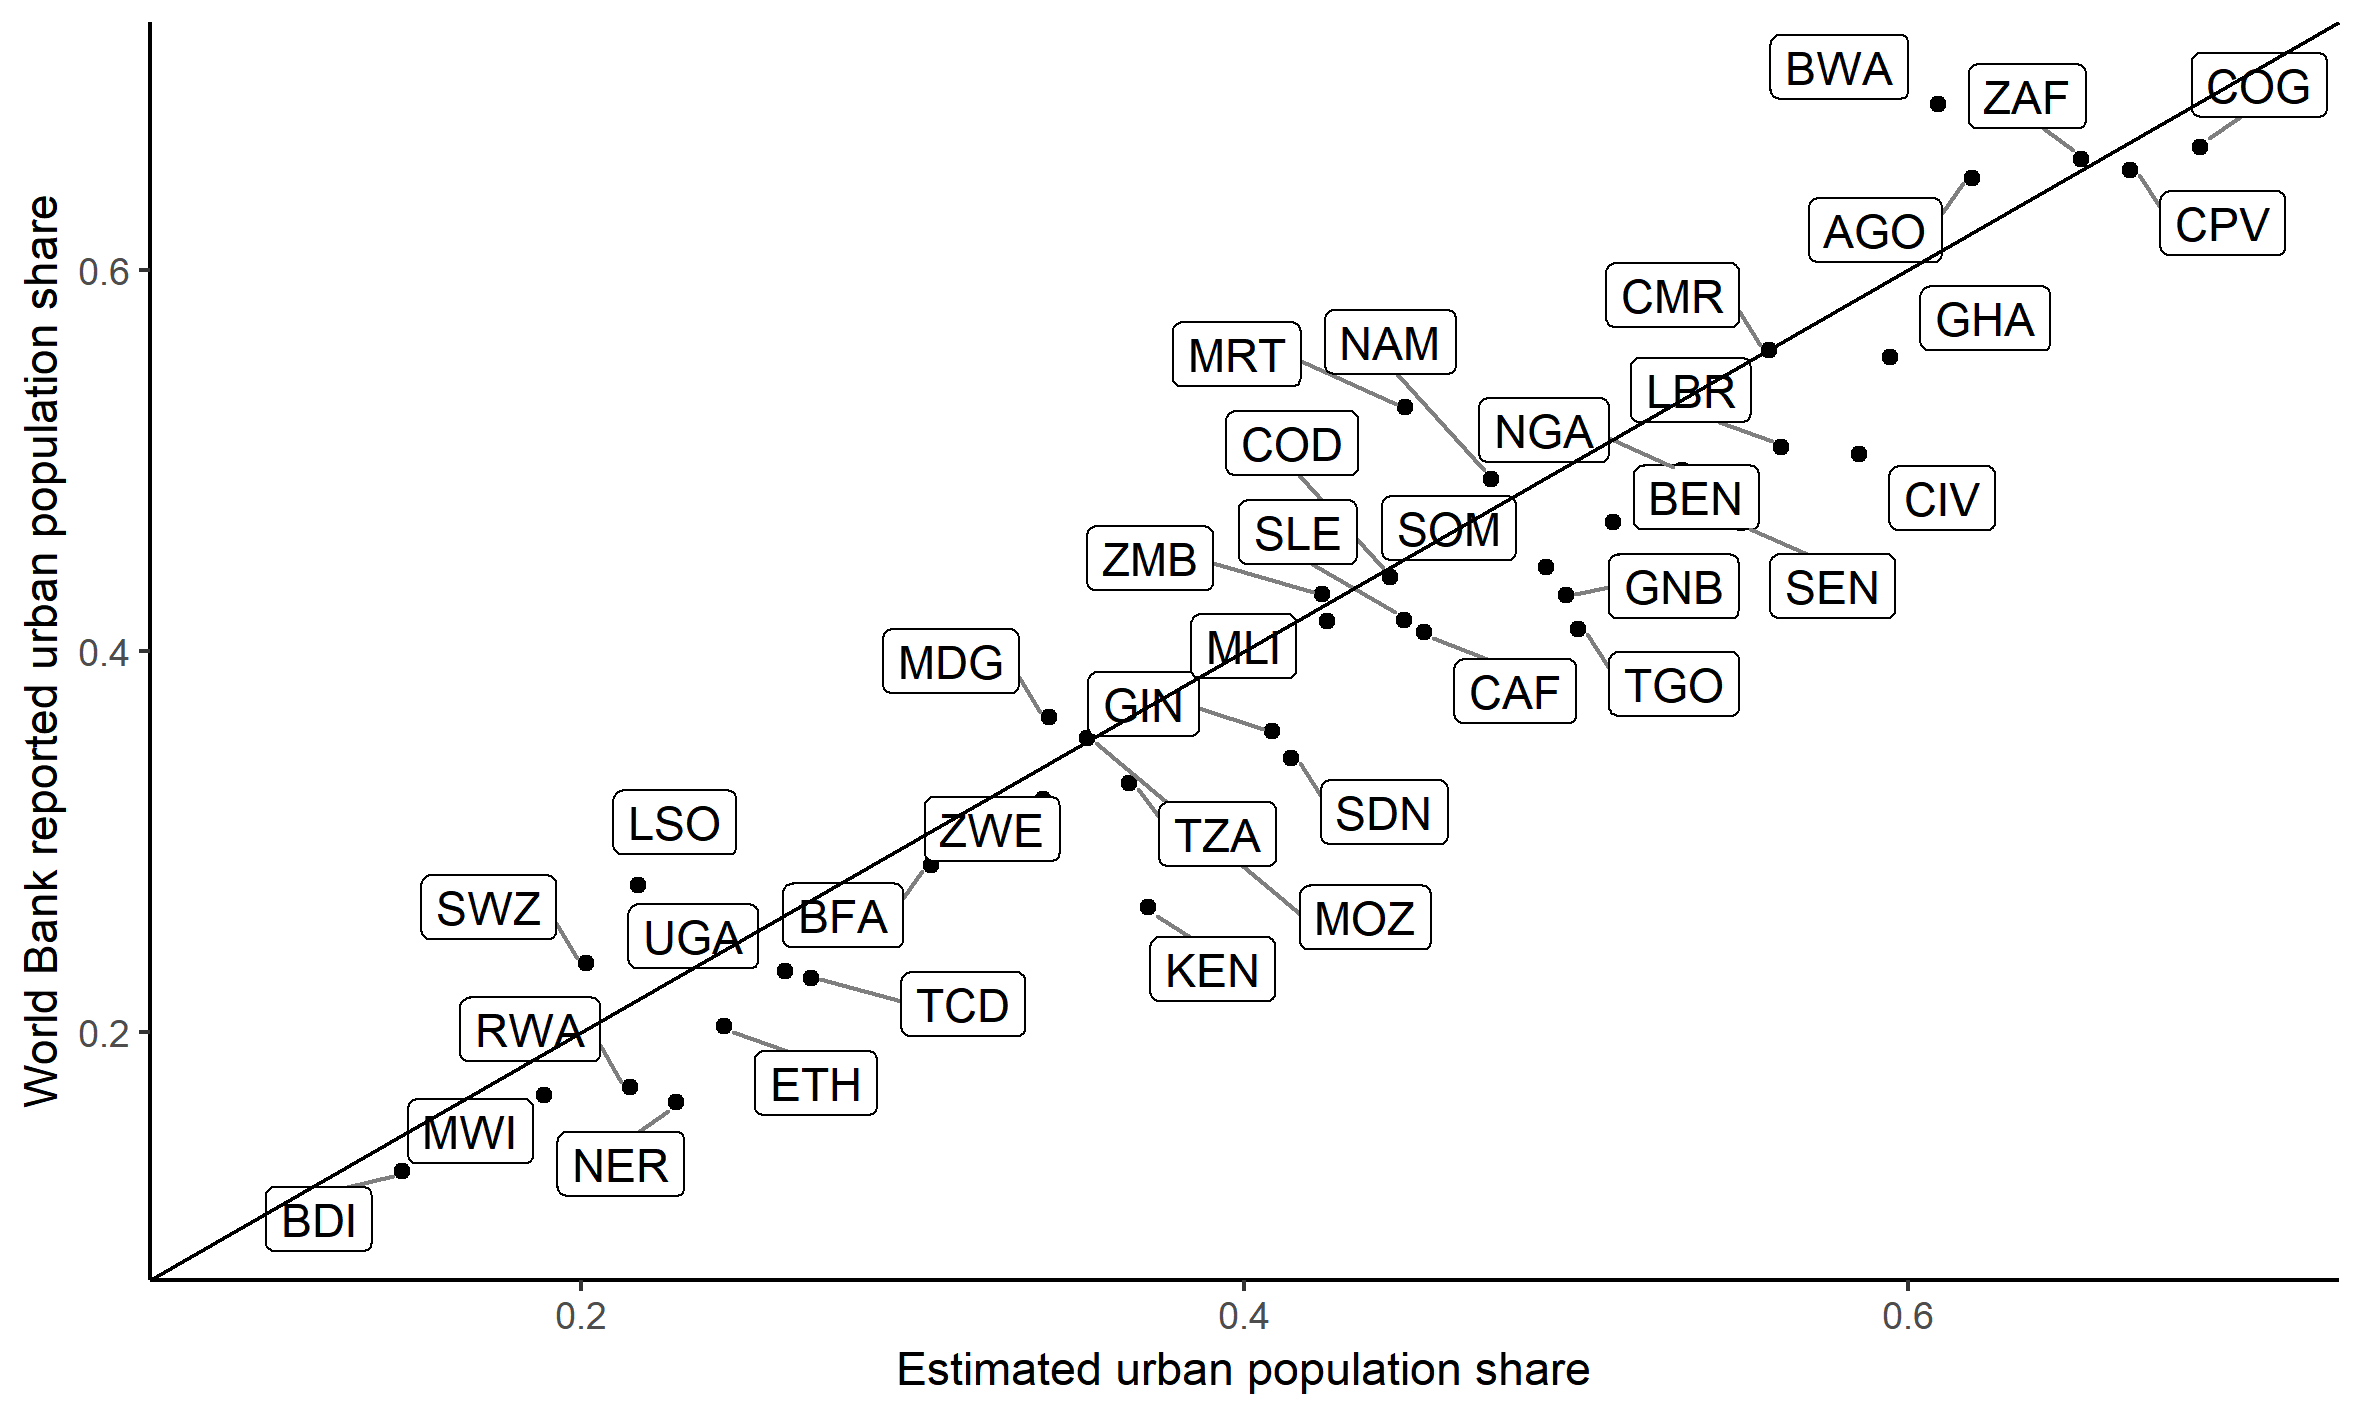
\includegraphics[scale=0.65]{figures/ruralvalid.png}
    \caption{Predicted vs. World Bank reported urban population share}
    \label{urvalid}
\end{figure}

The Google Earth Engine platform \citep{gorelick2017google} has been used to process spatially-explicit imagery and extract data which has subsequently been used to calculate trends, inequality, and to produce plots. The Data Access section links to the repository that hosts both Earth Engine Javascript code and R script and allows results reproduction, alteration of parameters for further sensitivity analysis, or further improvements. Results are also dynamically visualisable in an ad-hoc created web interface, under \url{http://electrificationmapping.shinyapps.io}. User-generated results can be also inputted in the interface, the source code of which is hosted on \url{https://github.com/giacfalk/Electrification_SSA_data/interface}.

Within the Earth Engine platform, the median value within each pixel of the VIIRS monthly composites has been calculated for both 2014 and 2018; a lower-bound noise floor has been set to $0.25 \mu W \cdot cm^{-2} \cdot sr^{-1}$ for 2014 and to $0.35 \mu W \cdot cm^{-2} \cdot sr^{-1}$ for 2018\footnote{The discrepancy in the noise caps is justified form the increased noisiness of the data witnessed from 2017, in all likelihood due to the alteration of a sensitivity parameter in the processing algorithm. The spread in the noise lower-bound cap has been determined from the examination of by-definition zero radiance pixels - such as within large water bodies - which nonetheless present a systematically positive radiance for data form 2017 onwards and a systematically zero radiance for previous data.} to remove calibration noise and emphimeral lights as discussed in the relevant literature \citep{roman_holidays_2015, levin_global_2017}; population counts within each GADM level 1 provinces have been produced for both people living in lit (above $0.25 / 0.35 \mu W \cdot cm^{-2} \cdot sr^{-1}$)  and in dark areas ($ \leq 0.25 / 0.35 \mu W \cdot cm^{-2} \cdot sr^{-1}$). The gridded 1$km^2$ classification has been used to aggregate results to different administrative scales (provincial and national) that are defined as spatial polygon features. Aggregation of the gridded data is achieved assuming grid cells belong to the polygon that contain its centroid. 

Inequality has been assessed by calculating the Gini index of electricity access among provinces within each country. Repeating the procedure between 2014 and 2018 allowed calculating the change in the distribution of the split in the 4-year period, as well as the corresponding change in the Gini index of within-country inequality in residential consumption. The Gini index measures inequality and it ranges between 0 and 1, where 0 expresses perfect equality and 1 is extreme inequality. It is defined as:

\begin{equation}
  G  = \frac { \sum _ { i = 1 } ^ { n } \sum _ { j = 1 } ^ { n } \left| x _ { i } - x _ { j } \right| } { 2 n \sum _ { i = 1 } ^ { n } x _ { i } }
\end{equation}

where $x$ is the electricity access of province $i$, $j$ are all remaining provinces, and $n$ is the total number of provinces. 

The definition of the Gini index is strictly related to that of the Lorenz curve \citep{lorenz1905methods}, defined as a continuous piecewise linear function $L(F)$, where $F$ defines the cumulative fraction of the population in the distribution (and is usually represented on the horizontal axis) and L represents the cumulative portion of the total response variable (in this case electricity acesss) and is plotted on the vertical axis.

With regards to estimated residential consumption levels, we considered a measure of per-capita radiance ($R_{pc}$) for those estimated to live in areas with electricity access (as recently showed in \citep{xiao2018spatio}). In particular, based on the distribution of the quartile values of non-zero per-capita light intensity across SSA countries (Figure \ref{distribution}), we defined four tiers of residential consumption at the median value of each quartile distribution. In order to account for the strong urban-rural discontinuity in terms of both consumption and population density, we did this separately for urban and peri-urban and rural settlements. Corresponding tier thresholds are reported in Table \ref{tiers}. 

\begin{figure}[!htb]
    \centering
    \subfloat[Urban]{   {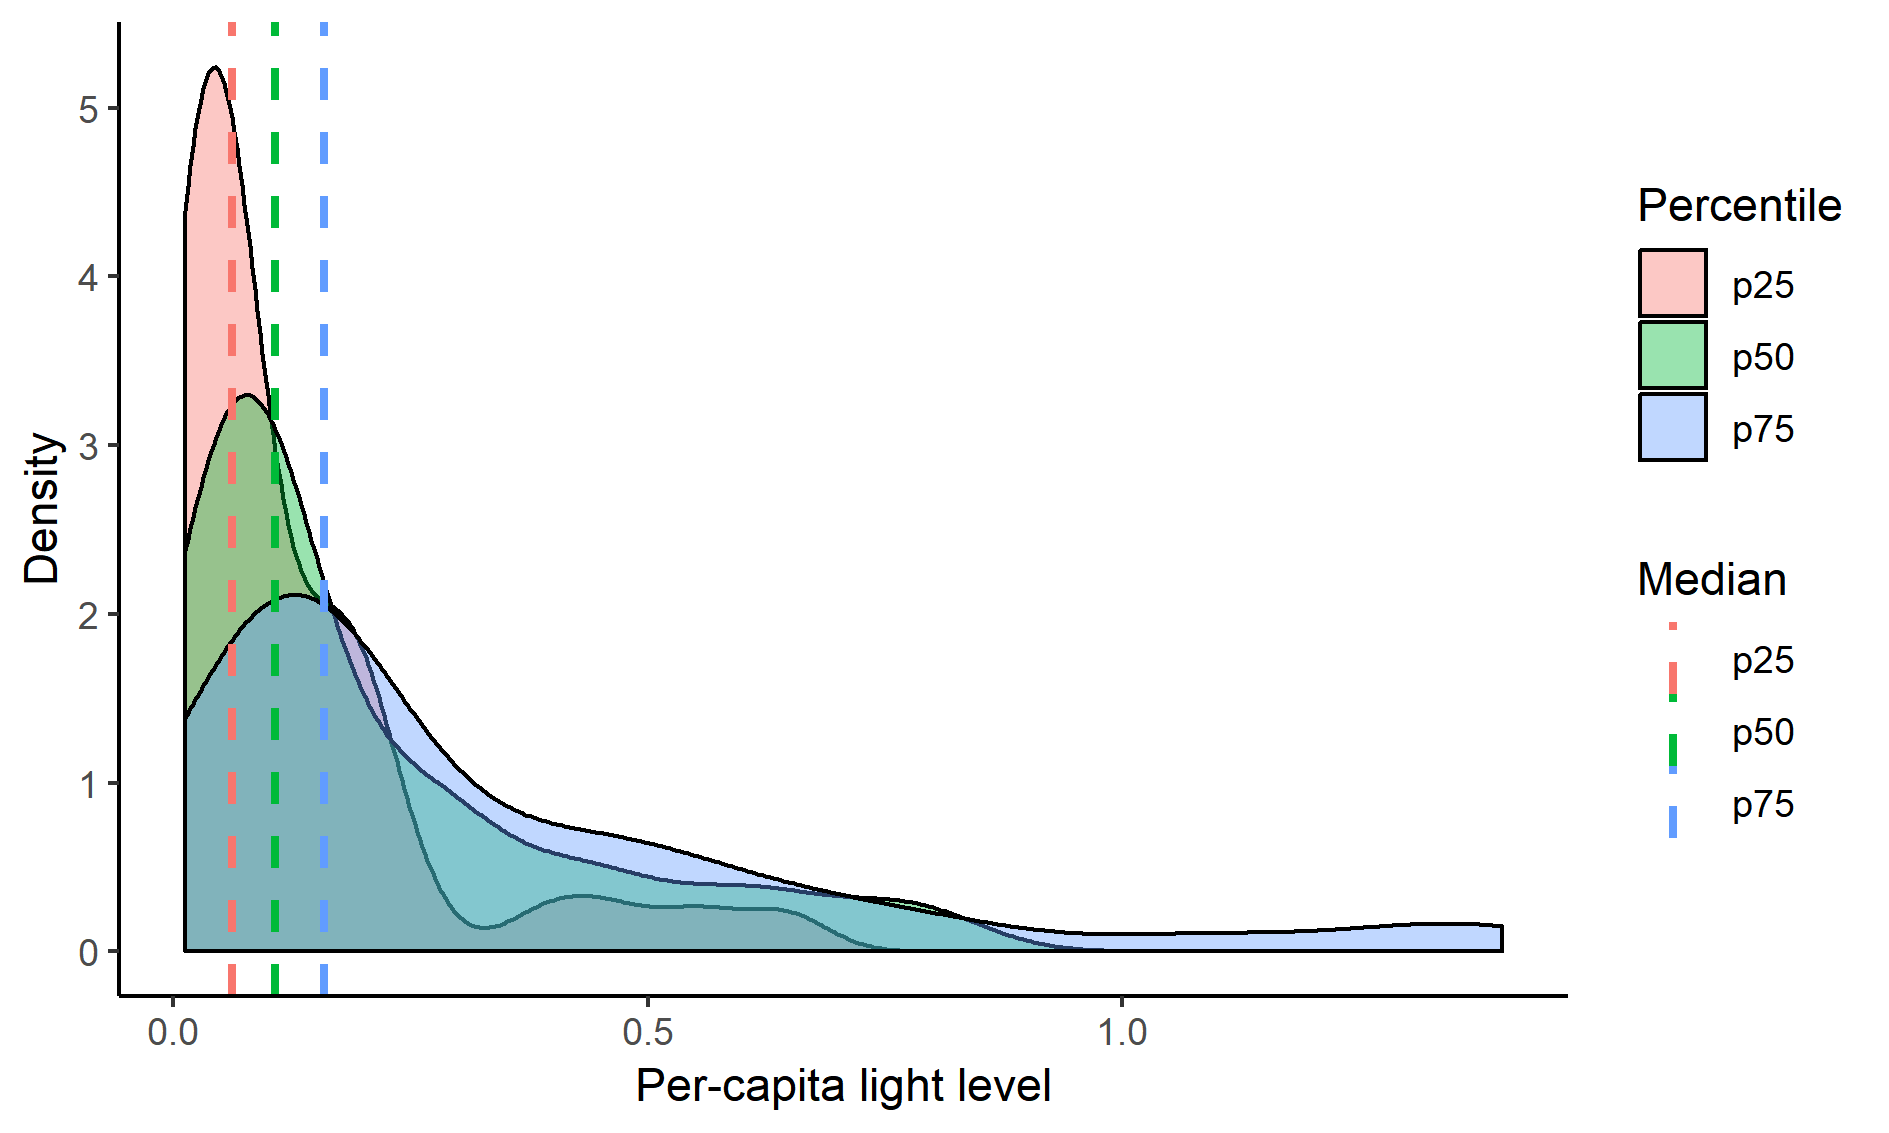
\includegraphics[scale = 0.65]{figures/histogram_urban.png} }}%
    \qquad
    \subfloat[Peri-urban and rural]{   {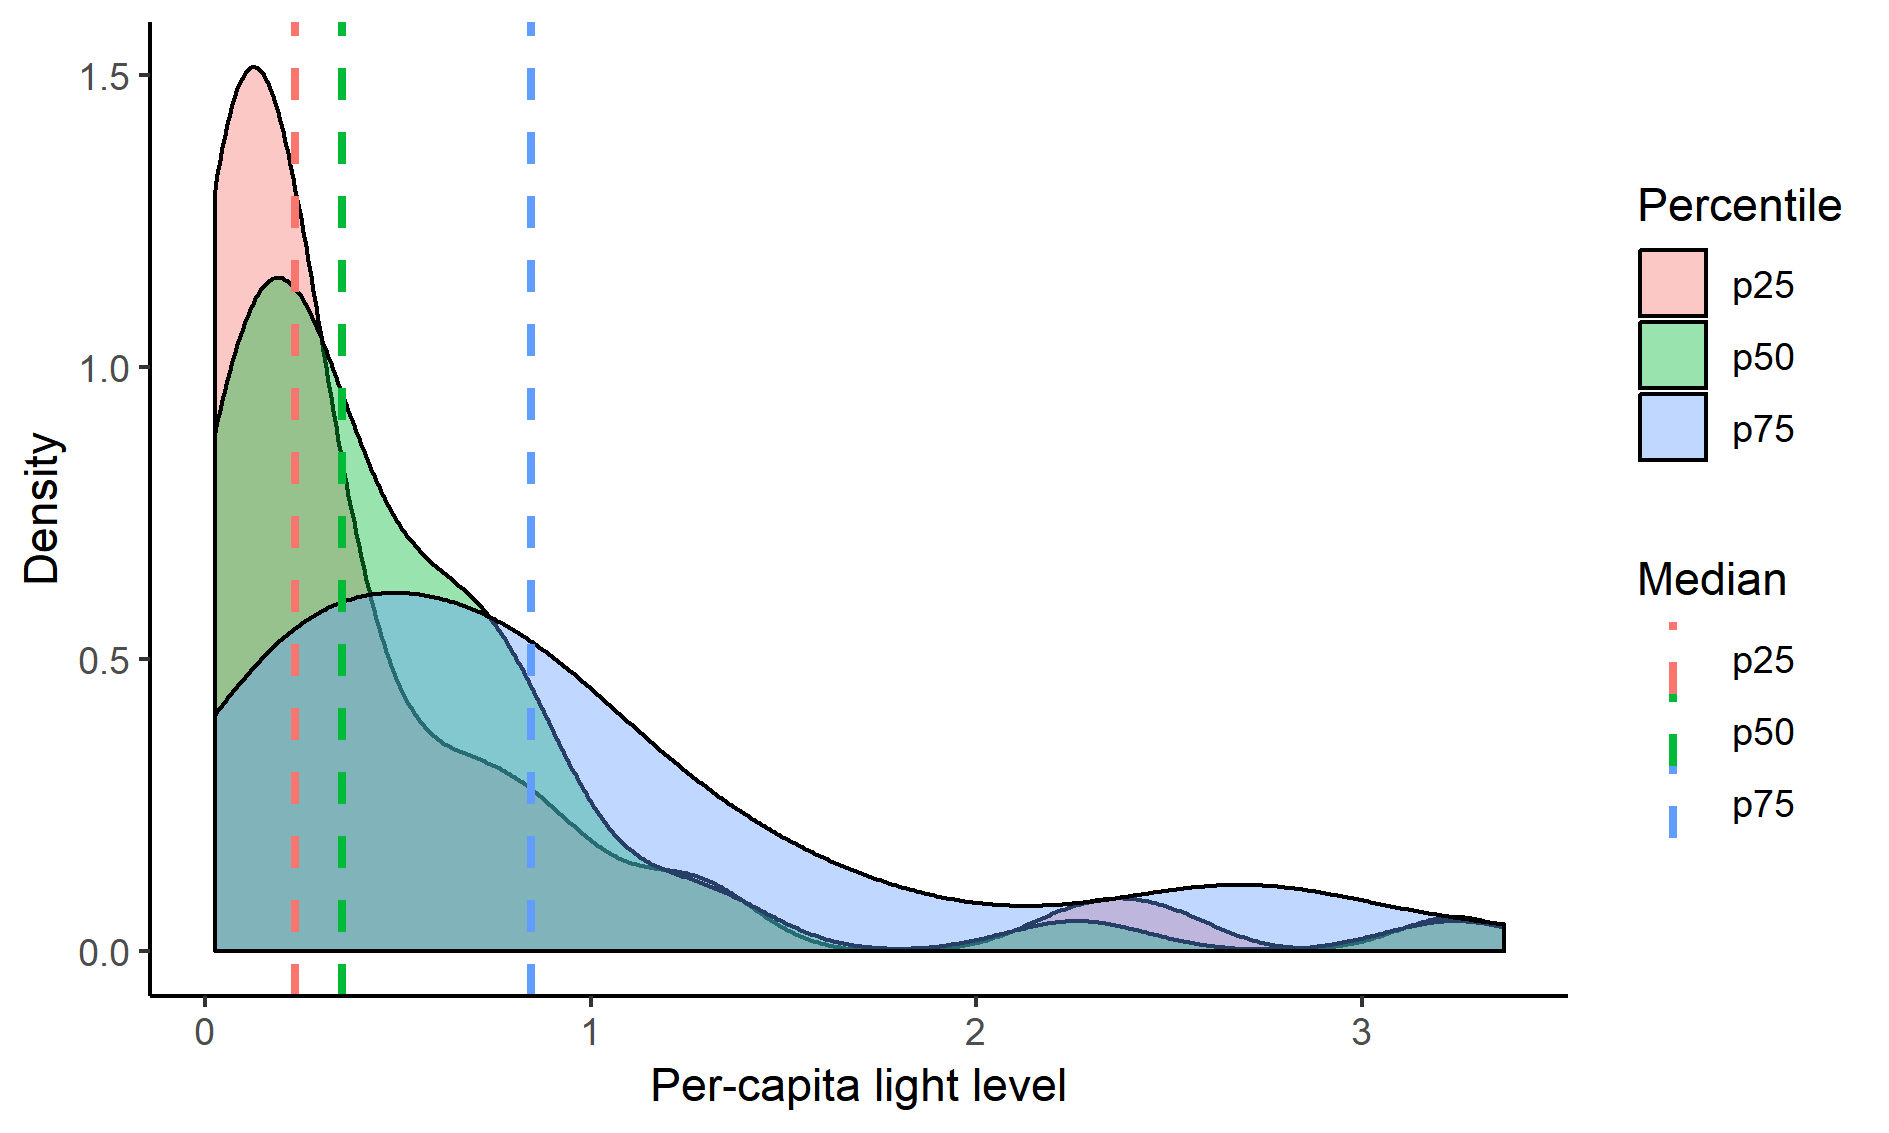
\includegraphics[scale = 0.65]{figures/histogram_rural.png} }}%
    \caption{Distribution of (non-zero) per-capita light intensity, median over all SSA countries}
    \label{distribution}
\end{figure}


\begin{table}[H]
\centering
\caption{Definition of tiers of per-capita light intensity in electrified areas}
\small
\label{tiers}
\begin{tabular}{@{}c|cc|cc@{}}
\hline  \hline
\multirow{1}{*}{\bfseries} & 
\multirow{1}{*}{\bfseries Urban} & 
\multirow{1}{*}{\bfseries} & 
\multirow{1}{*}{\bfseries Rural}\\ \hline
Tier & Lower-bound & Upper-bound & Lower-bound  & Upper-bound \\ \hline
1  & $>0$ & $<0.06$ & $>0$ & $<0.38$  \\
2  & $\geq0.06$ & $<0.11$ &$ >0.38$ & $<0.66$\\
3  & $\geq0.11$ & $<0.16$  &$>0.66$ & $<1.63$\\
4  & $\geq0.16$ & - & $>1.63$ & - \\ 
\hline
\end{tabular}
\end{table}

Based on the four tiers, the population in electrified areas was summed for each level of residential consumption in both urban and peri-urban/rural areas, and the relative share of tiers in each country was calculated. Finally, estimates have been used to identify electrification hotspots, defined as (i) provinces with robustly increasing population without access - undermining electricity access rates growth; (ii) areas which have been experiencing a rapidly growing demand, and (iii) areas with high nominal access rates but very low estimated per-capita residential consumption, respectively. 

A general caveat of the approach to the data generation and analysis is that it was assumed that a pixel being lit implies that everyone in that location has access. While this could be a 'naive' assumption and the main reason for the discrepancy in the validation stage, it nonetheless implies that those people are in proximity of connection possibilities, i.e. remoteness is not a significant problem. This suggests that in those areas the challenge is that of fostering access with enabling policy for financially constrained households, rather than a need for infrastructure development  At the same time, a pixel being identified as dark still allows for the possibility of some form of (standalone) electricity generation is in place. In the latter case, either the lighting component of total final electricity consumption is very scarce, or the actual installed capacity and power output is negligible.  Other important sources of uncertainty for the analysis include (i) the accuracy of official electrification rates; (ii) our choice of the nighttime light noise floor; (iii) the accuracy of the gridded population data across different years. For instance, large urban areas, detected as entirely lit, might still host a significant number of people who are not (at least officially) connected to the grid. Such reasons underpin the importance of the publication of the source code to allow results alteration as more recent, improved local data for validation becomes available. Furthermore, Section \ref{sensitivity} reports the results of sensitivity analysis to address sources of uncertainties (ii) and (iii). 

\section{Validation}
To assess the consistency of the new dataset of electrificaiton rates, we produced a cross-sectional fit representing the NTL estimate against the most recent data source available, the 2016 ESMAP/World Bank \textit{Tracking SDG 7} electrification rates data, as shown in Figure \ref{ntlesmap}. Overall, this reveals a rather consistent estimation of the heterogeneity in the data, although discrepancies are identified. The remote sensing approach performs well in terms of reproducing the electrification rates in Botswana, Ghana, Sudan, Congo, Somalia, and Burundi. The largest discrepancies are found for Eritrea (-39\%), Ethiopia (-29\%), Equatorial Guinea (-35\%), and Cameron (-22\%), Malawi (+12\%), Liberia (+17\%), and Guinea Bissau (+15\%). Upaward discrepancies (overestimations) are prone to be (at least partially) attribuatable to the issue of illegal connections (refer to \citep{de2018kenya, yakubu2018electricity} for recent contribution and estimations of electricity thefts) or to \textbf{other sources of light from e.g., gas flaring}. Downward bias can be attributed - among others - to the missed detection from NTL of standalone solutions such as solar-home-systems, or to the low level of lighting among highly distributed communities. 

\begin{figure}[H]
    \centering
    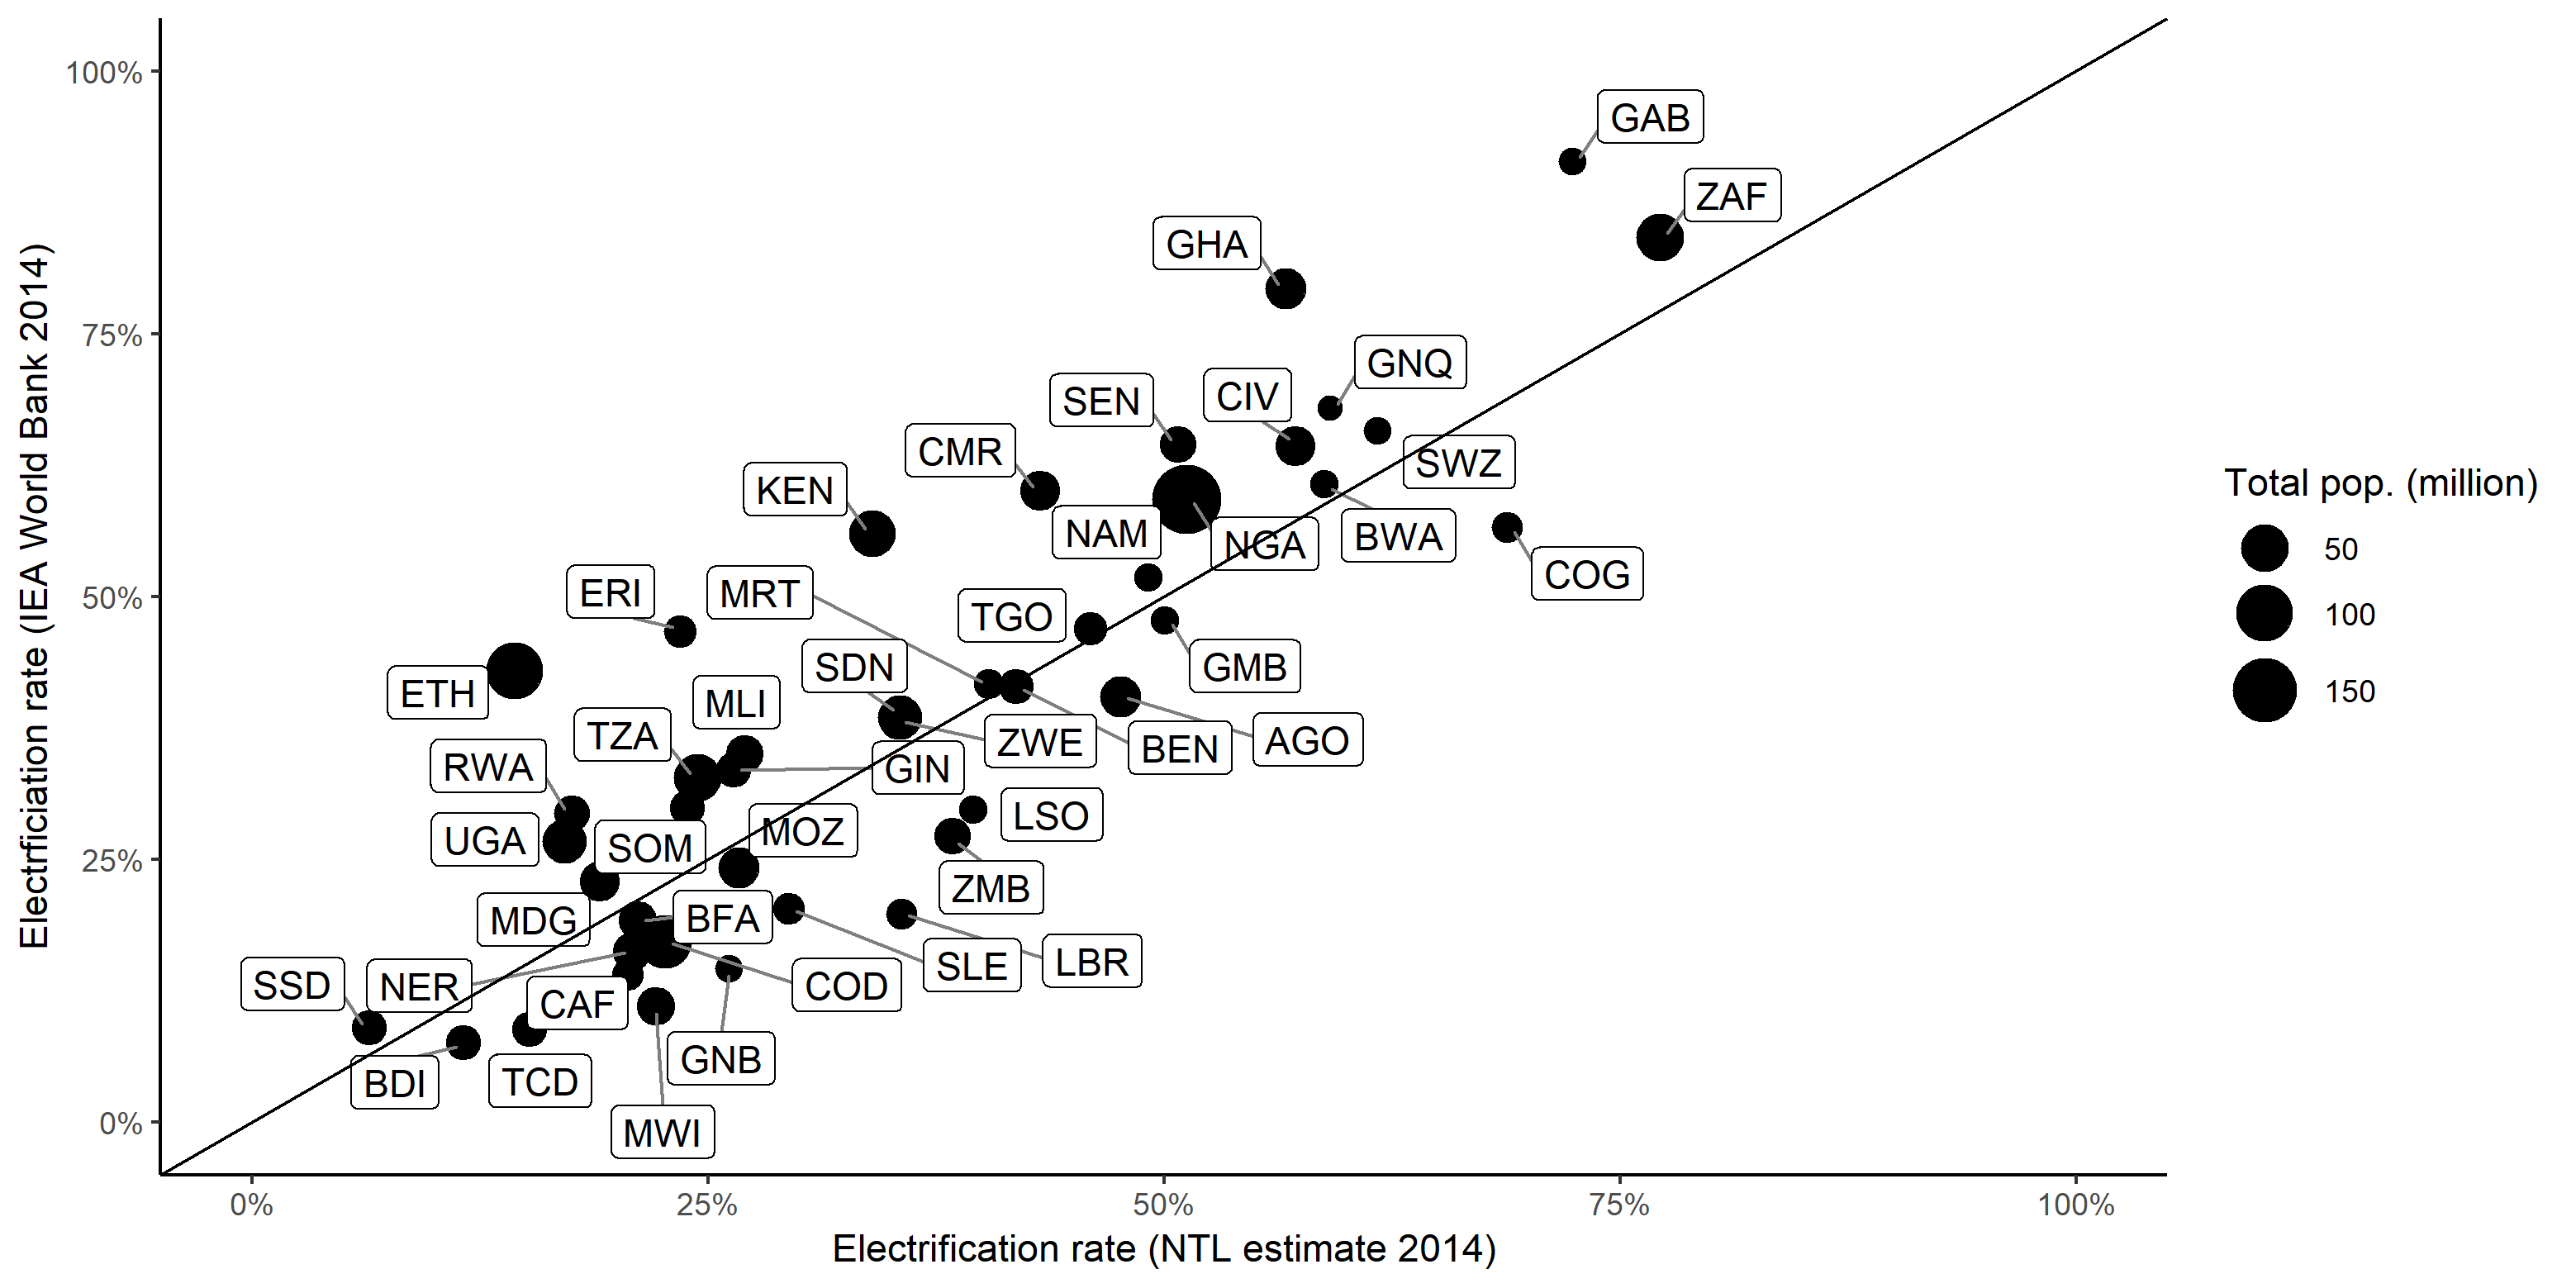
\includegraphics[scale=0.5]{figures/comparisonwb.png}
    \caption{NTL estimate for 2016 vs. ESMAP/World Bank 2016}
    \label{ntlesmap}
\end{figure}

Overall, the validation shows that our bottom-up approach to estimate electrification rates - derived from 1-$km^2$ grid cell level estimates - represents an effective method for predicting national electrification rates. In an attempt to perform a more precise validation, we collected survey-derived province-level shares of households with access to electricity from the DHS Program STATcompiler (including demographic and health surveys and disease-related surveys). This was possible for fifteen SSA countries (Angola, Burundi, Burkina Faso, DR Congo, Ethiopia, Ghana, Mali, Malawi, Mozambique, Nigeria, Senegal, Sierra Leone, Tanzania, Zambia, and Zimbabwe). It must be noted that the the surveying period of data reported by the DHS STATcompiler often spans between two calendar years. Therefore, in order to produce a consistent validation, we had to refer to different years (between 2014 and 2017) depending on the surveying year in each country and produce NTL-based estimates for each year. Hence, given the variety of sources, the following comparison serves a general consistency validation. Also, DHS data is subject to smoothing processes due to the use of sampling weights, which might result in inaccurate overall access rates estimates \citep{macro2009measure}. 

\begin{figure}[H]
    \centering
    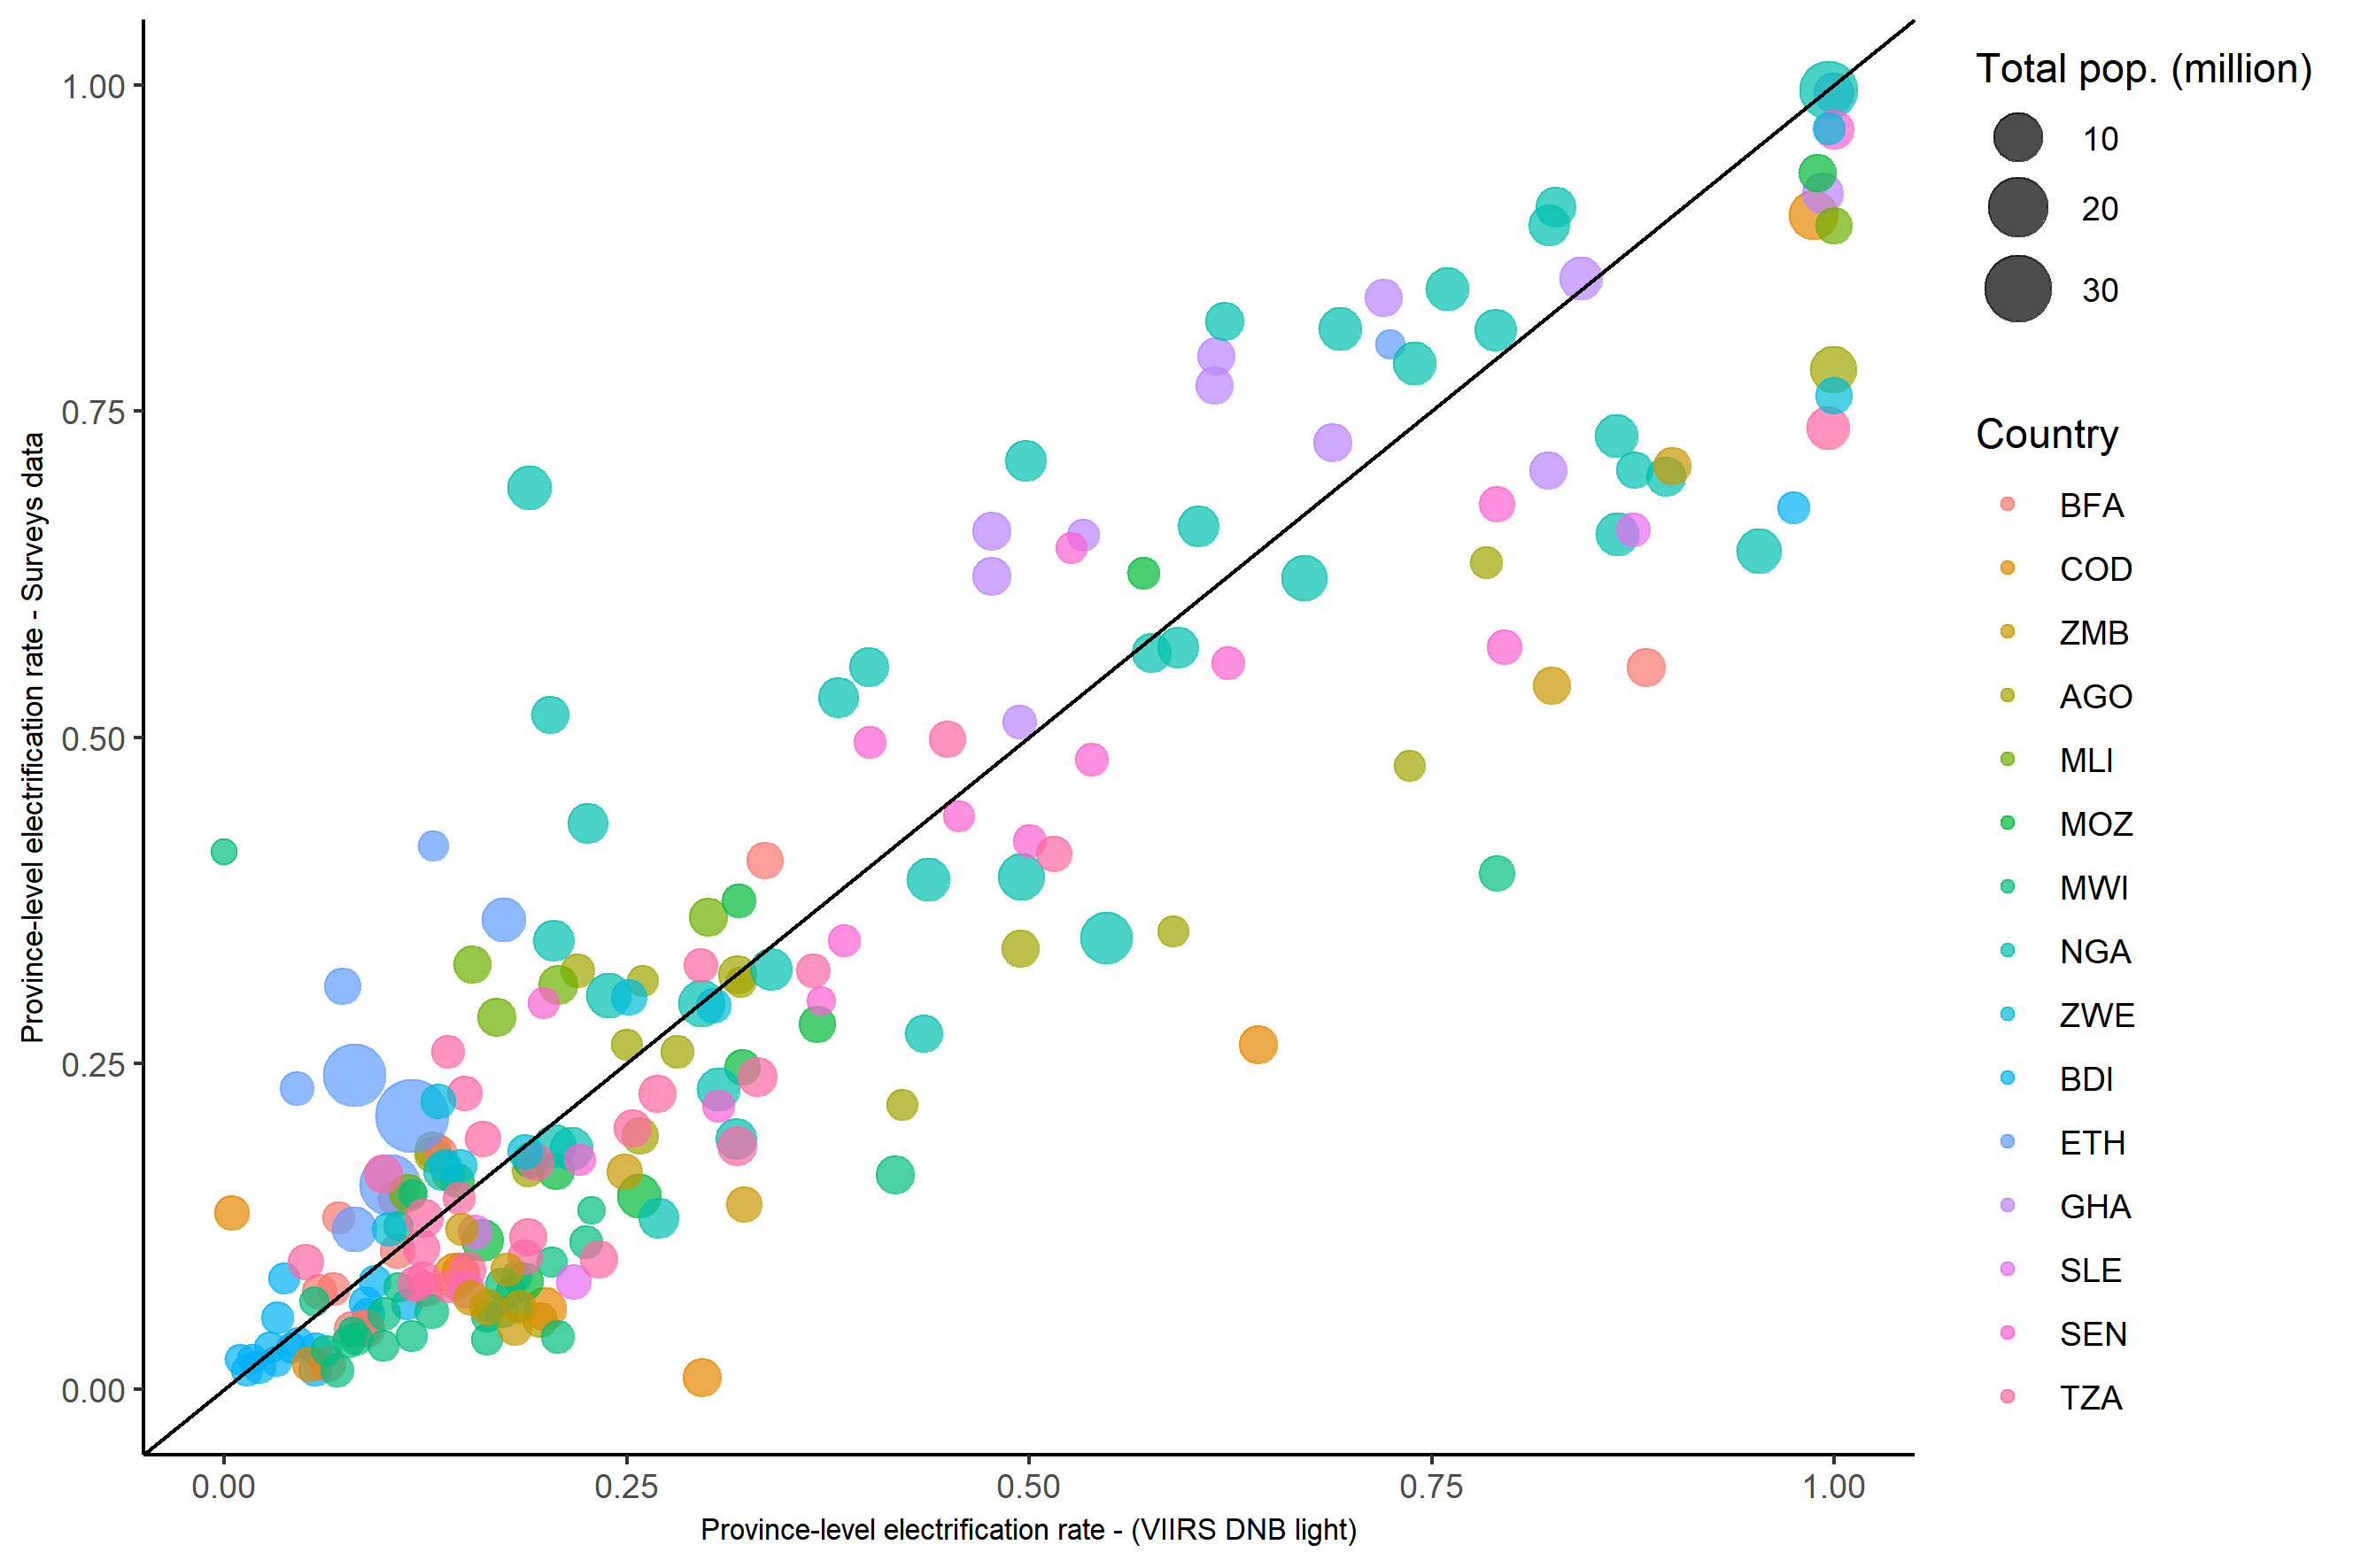
\includegraphics[scale=0.7]{figures/comparisontanzaniazoom.png}
    \caption{Province-level electrificaiton: consistency validation}
    \label{TanzaniaNigeriaGhana}
\end{figure}

Our methodology is found to be generally consistent with the specific electrification rates, as shown in Figure \ref{TanzaniaNigeriaGhana}, although some inconsistencies are found.

With regards to validating the estimate of the actual residential consumption levels, the challenge is even greater, due to scarcity of data at a precise and high enough spatial scale. The approach that we adopted was based on retrieving the location and characteristics of operating mini-grids in Tanzania published by the WRI, assessing the total intensity of light over the 500m buffer at the mini-grid reported location, and compare it with the nameplate stated capacity of such mini-grids. Figure \ref{mg} reports the results of such analysis in log-log terms (due to heterogeneity in the scale of the two variables, with many low capacity facilities and few larger ones). It shows three main results and caveats: first, a positive link between the two variables is observed; second, the NTLs appear to be better at predicting the mini-grids' capacity above a minimum threshold (of around 1 MW); third, capacity is nameplate, and there is no available data to assess the effective functioning, amount of generation, and precision of reported location of such sites. Nonetheless, the comparison provides useful insight into the performance of the dataset to track electricity sector development.

\begin{figure}[H]
    \centering
    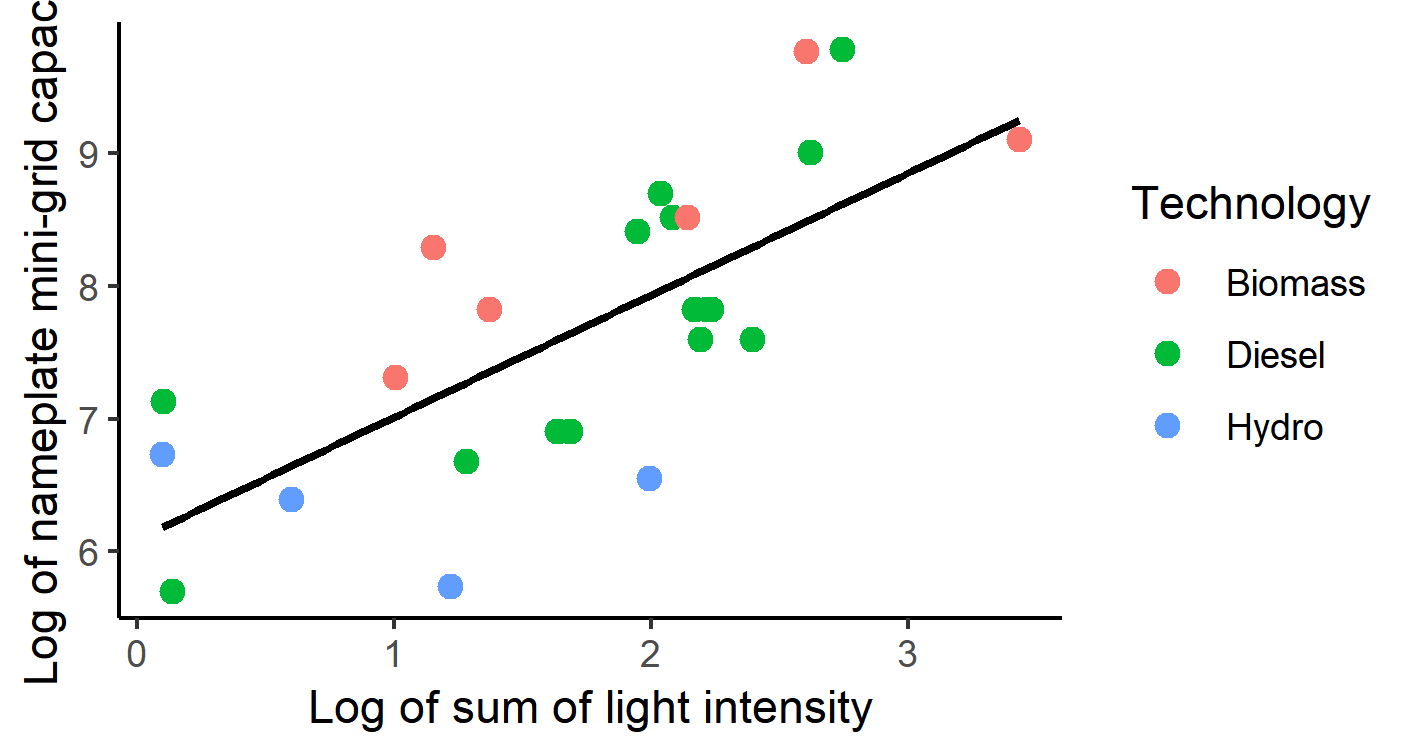
\includegraphics{figures/mgtza.png}
    \caption{Minigrids in Tanzania to validate (log) sum of light intensity as a proxy of power consumption}
    \label{mg}
\end{figure}

\subsection{Sensitivity analysis} \label{sensitivity}
Figure \ref{ntlesmap2} show a validation plot similar to that reported above, except it includes three points for each country. These shows the change in the estimate in response to a $\pm25\%$ change in the nighttime light data noise floor, and can be interpreted a as a confidence interval for the estimate. Although the accuracy of the estimates are heterogeneous across countries for the three noise floors, a simple linear regression yields an $R^2$ of 0.77 for the baseline, of 0.76 for the $+25\%$, and of 0.78 for the for the $-25\%$. 

\begin{figure}[H]
    \centering
    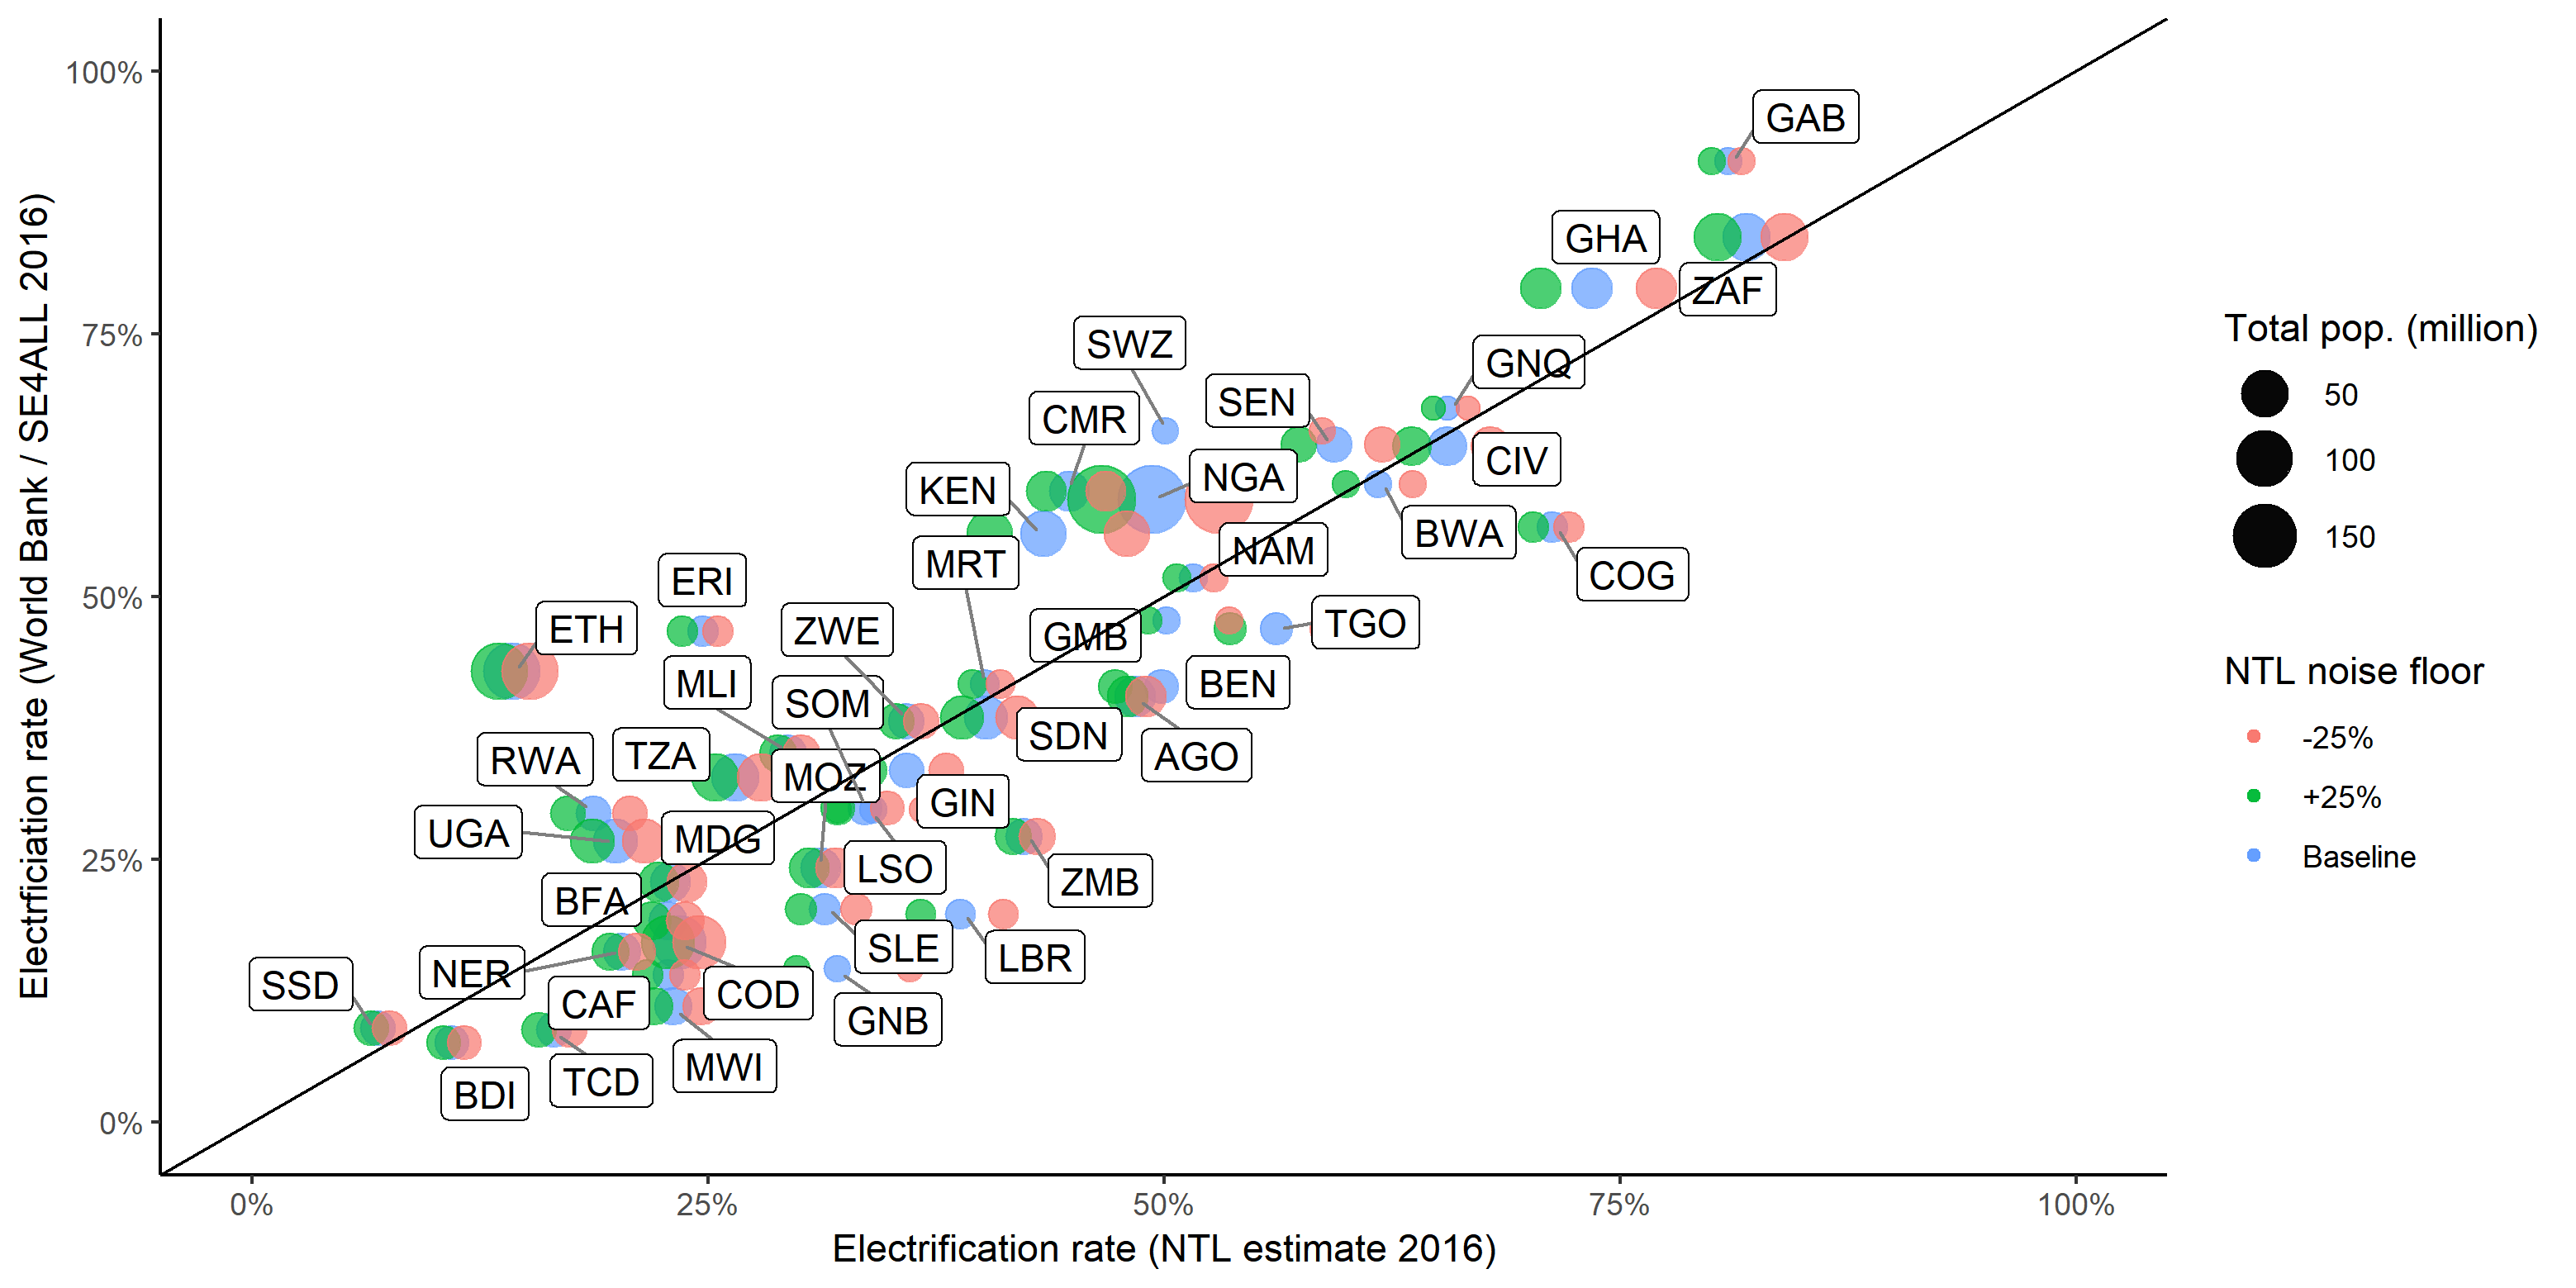
\includegraphics[scale=0.5]{figures/sensitivity_noise.png}
    \caption{Sensitivity analysis for country-level electrification rates estimate validation}
    \label{ntlesmap2}
\end{figure}

To provide a sensitivity check over the gridded population data, we reproduced validation also over the WorldPop dataset.  Figure \ref{ntlesmap3} compares the results obtained with LandScan and WorldPop data. For national electrification rates, the LandScan results in a \textit{ceteris paribus} significantly more accurate prediction than the WorldPop. A simple linear regression produces a $R^2$ of 0.77 for the LandScan and of 0.63 for the WorldPop data. Therefore, results underpin the choice of using LandScan as the default gridded population.\footnote{Nonetheless, it is sufficient to alter one line of the code to replicate all the following steps with a different population dataset.}

\begin{figure}[H]
    \centering
    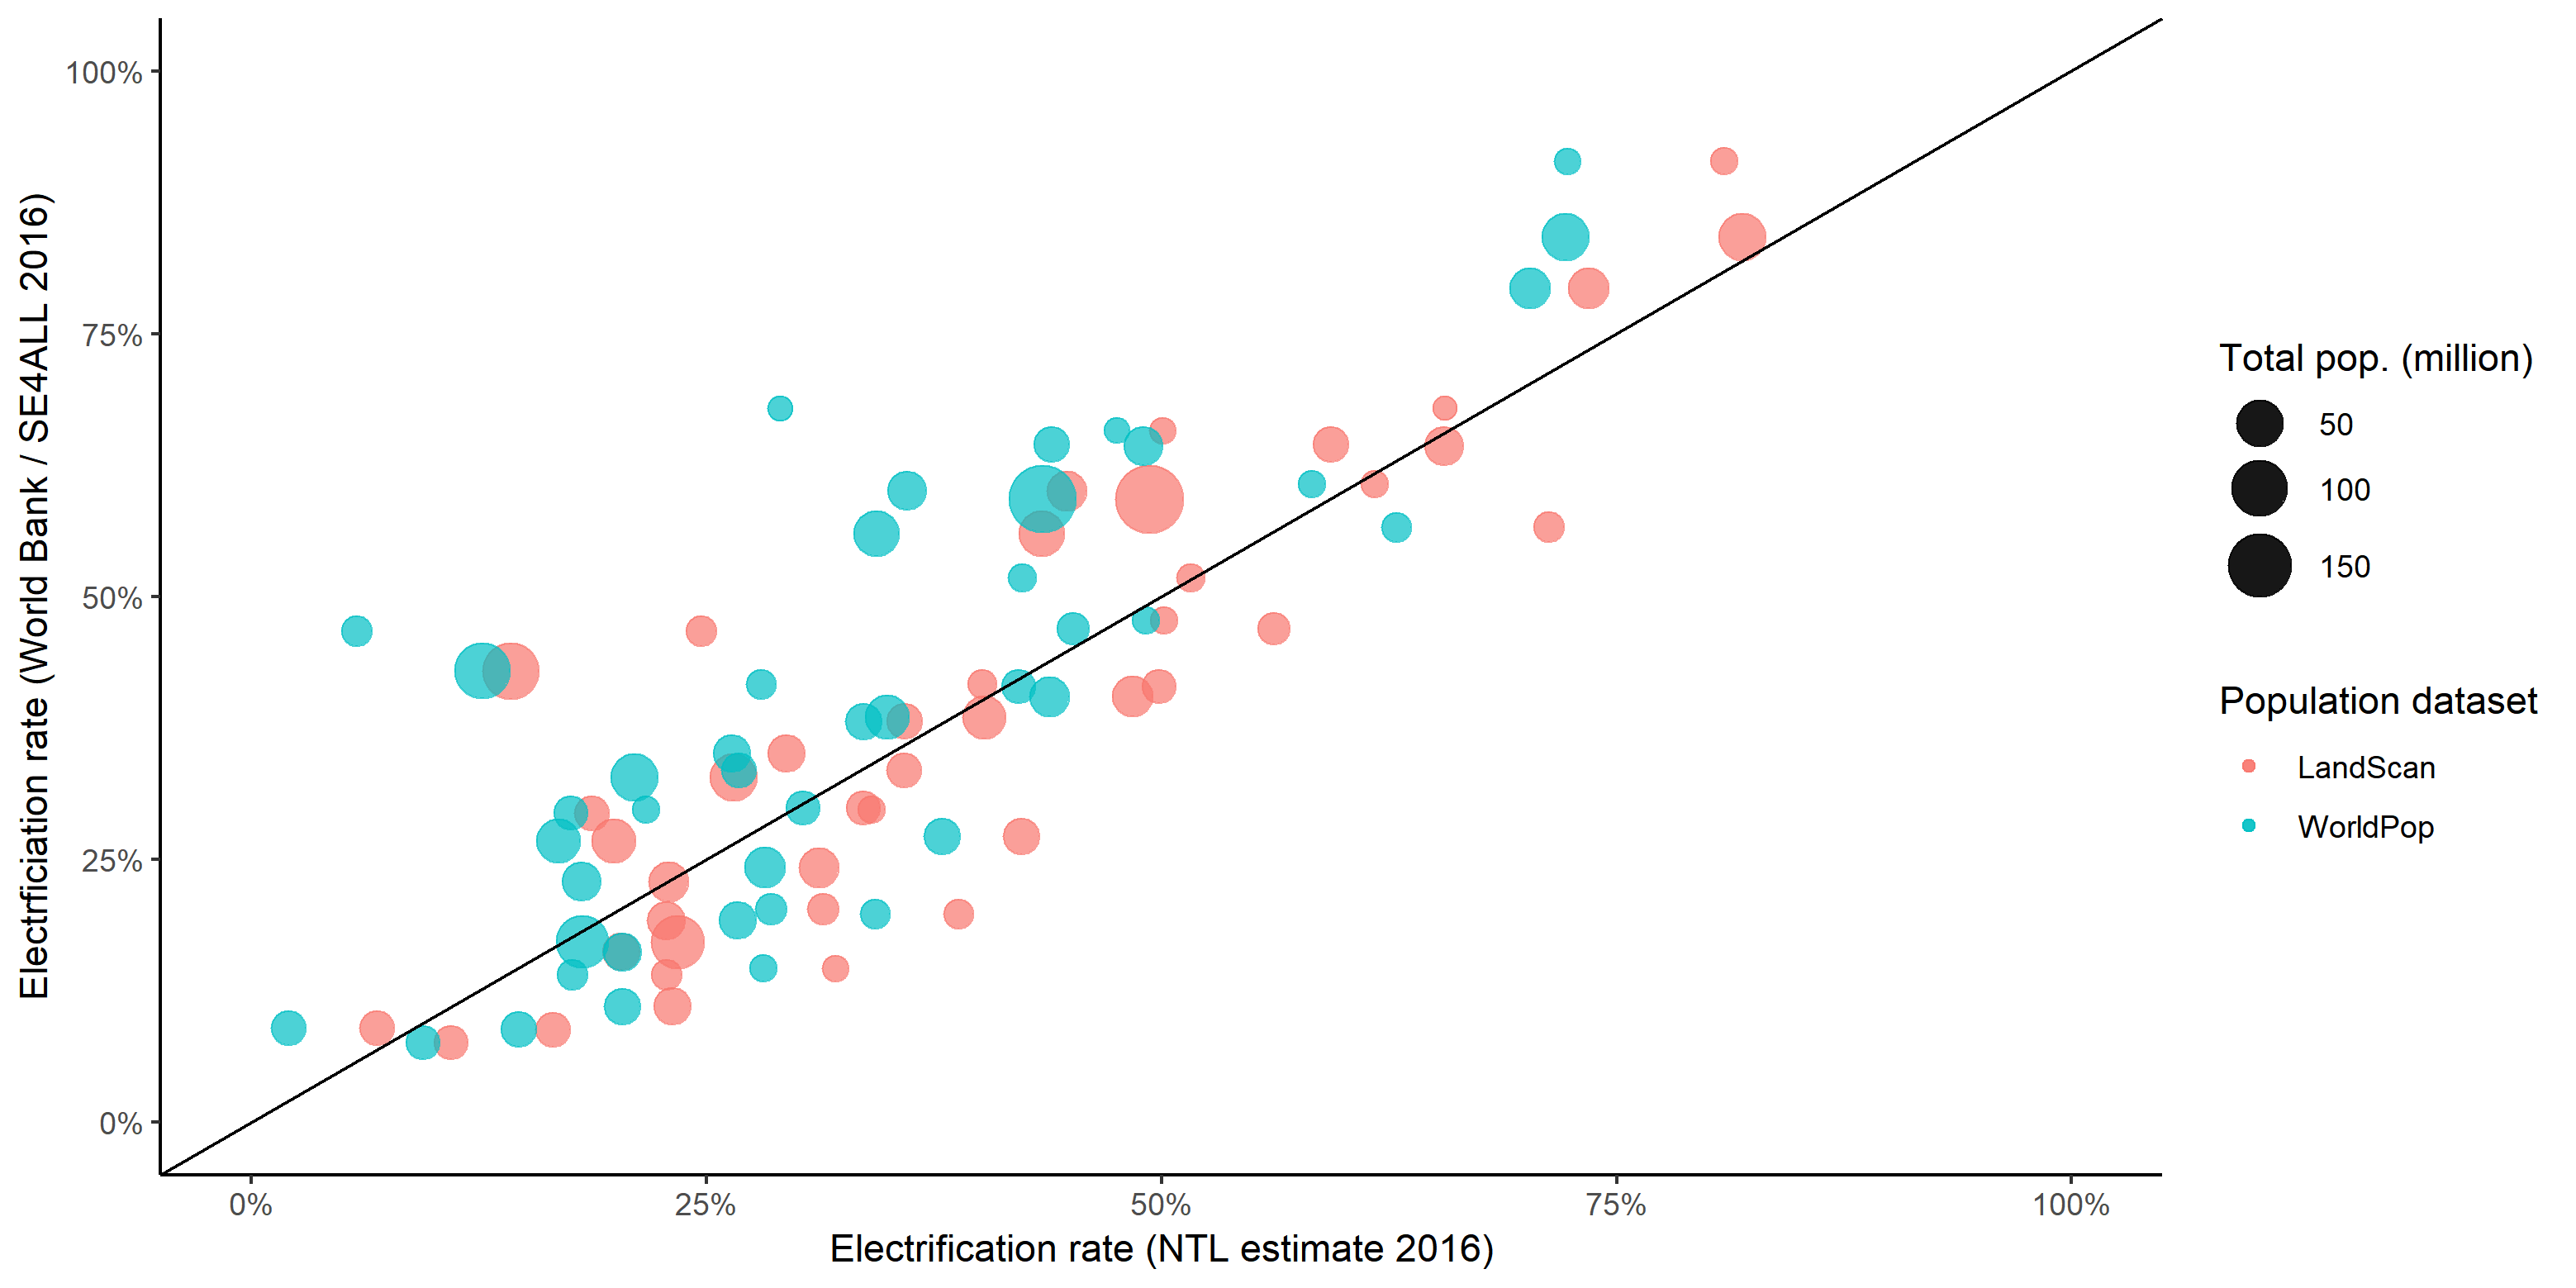
\includegraphics[scale=0.5]{figures/sensitivity_population.png}
    \caption{Population datasets comparison for country-level electrification rates estimate}
    \label{ntlesmap3}
\end{figure}

\section{Results}
\subsection{Trends in electrification across and within countries}
Figure \ref{barplot} shows the estimated electrification efforts by country between 2014 and 2018 and the effective electrification rate attained in 2018. Ghana results as the country with the steepest growth rate in the period under examination, at +27.5\%. It is followed by Kenya (+20\%) and Benin and Togo (+18\%). Other countries - crucially the already little electrified Burundi, Democratic Republic of the Congo, and Chad, but also Ethiopia and Niger - show very little progress, below +2.5\%.

\begin{figure}[H]
    \centering
    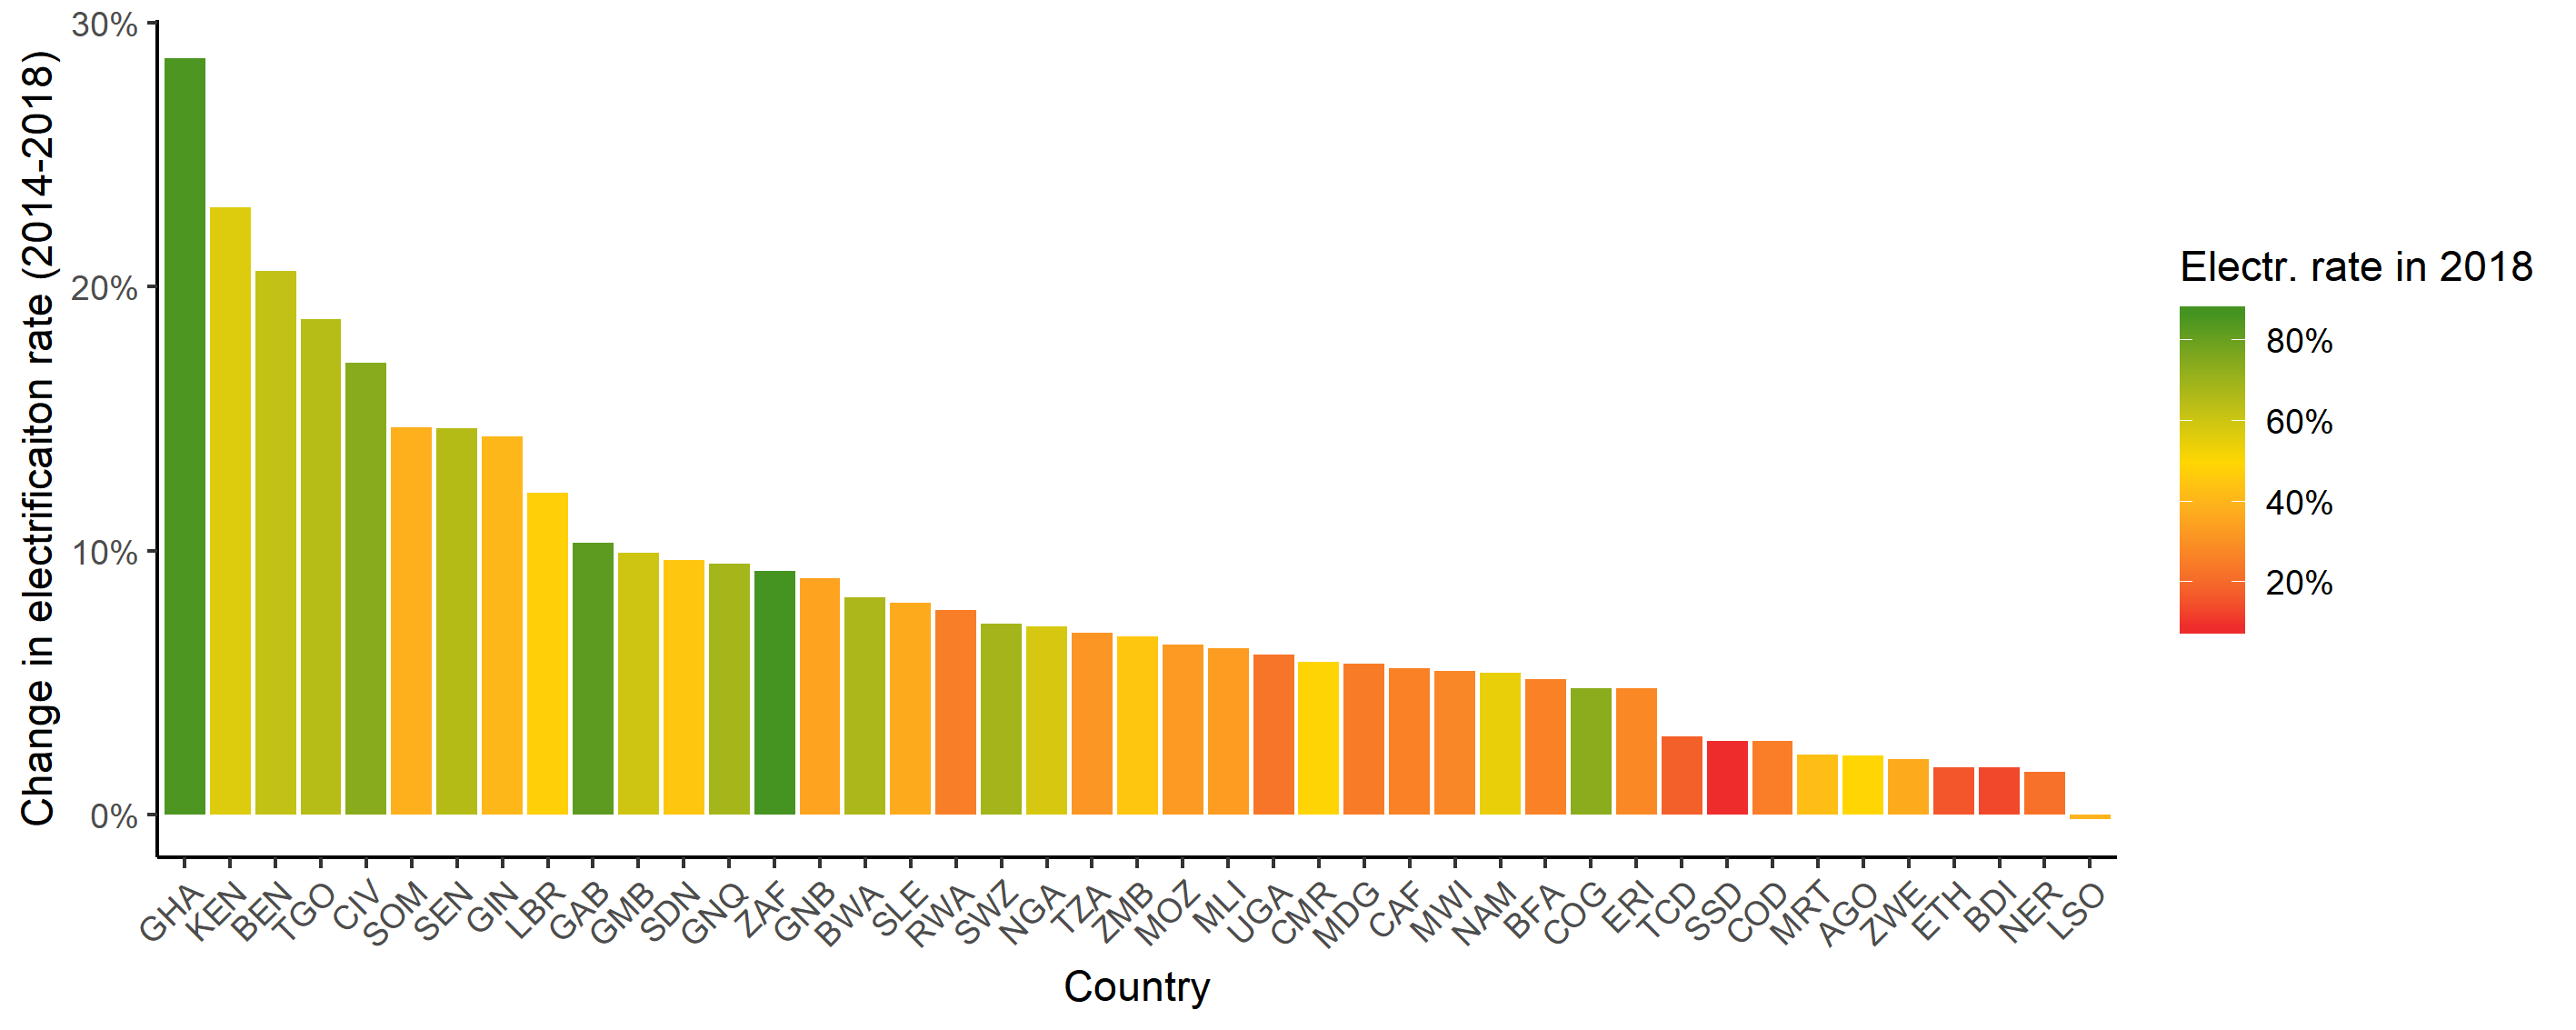
\includegraphics[scale=0.7]{figures/barplot.png}
    \caption{Electrification efforts (2014-2018)}
    \label{barplot}
\end{figure}

\subsection{Inequality assessed}
The Gini index of electricity access inequality among the provinces of each country - calculated for both 2014 and 2018 - is plotted Figure \ref{maps}a.  In a similar fashion, Figure \ref{maps}b shpws the Gini index of residential consumption inequality at a national scale, defined as the inequality in residential consumption among the national population with access (see Sect90j 4.3). 

\begin{figure}[H]
    \centering
    \subfloat[Access Gini]{{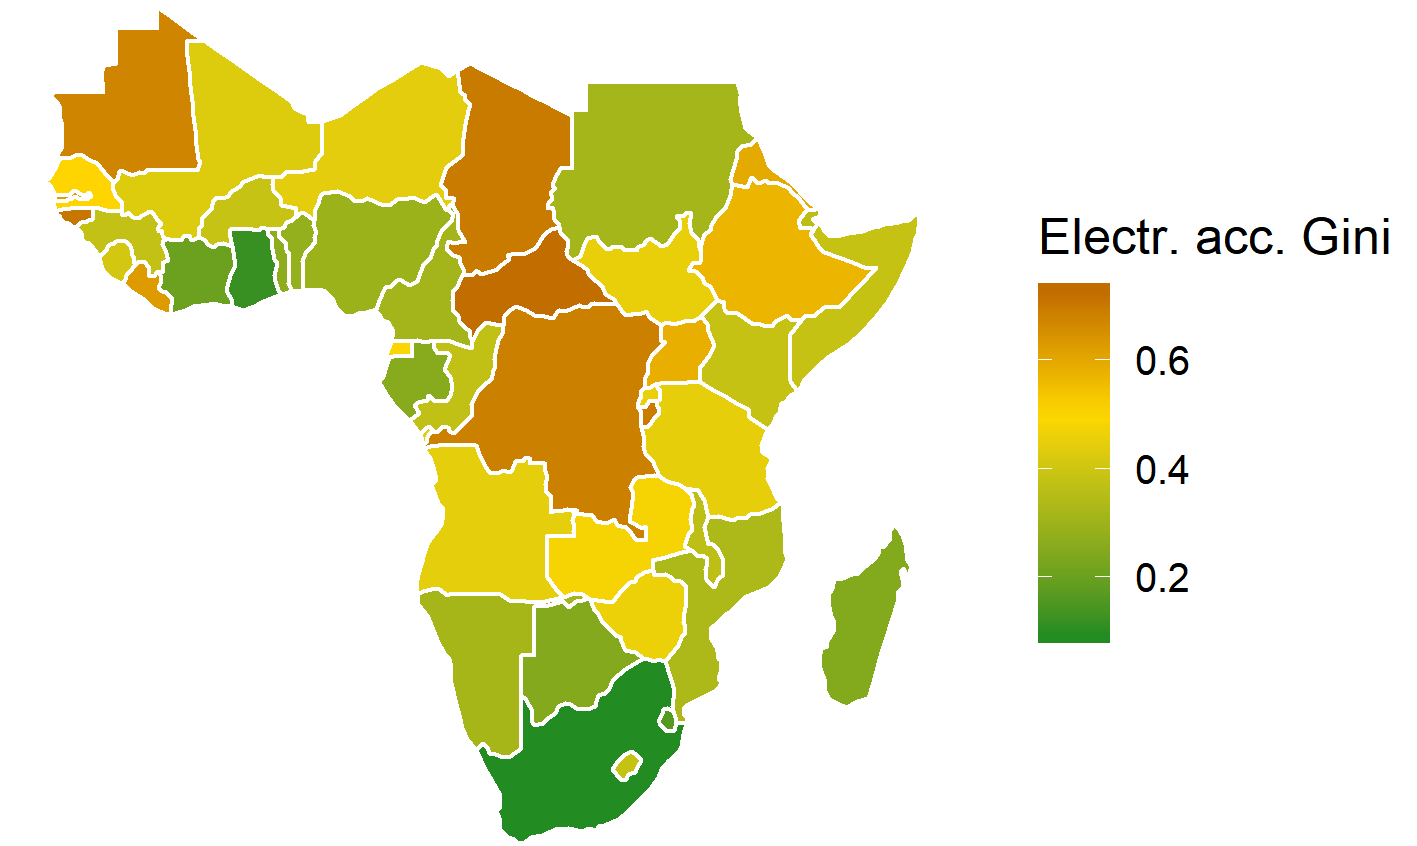
\includegraphics[scale=0.5]{figures/mapginiaccess.png} }}%
    \qquad
    \subfloat[residential consumption Gini]{{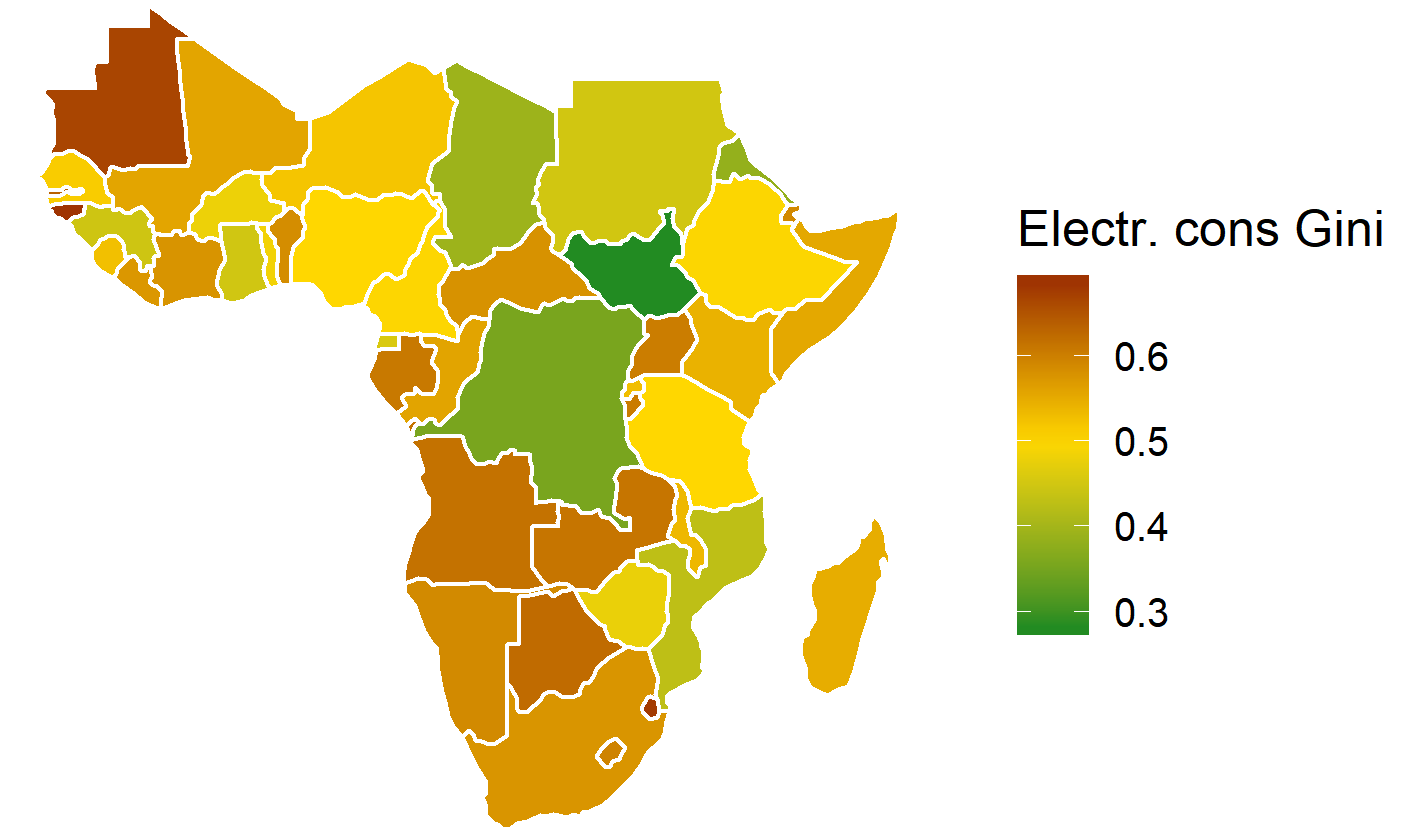
\includegraphics[scale=0.5]{figures/mapginicons.png} }}%
    \caption{Electricity access and residential consumption Gini indexes for 2018}
      \label{maps}
\end{figure}

Lorenz curves provide a further insight into the within-country inequality in electricity access. Figure \ref{lorenz} plots - for a selected number of countries - the cumulative share of provinces and the corresponding electrification rates. The functional form and the presence of discontinuity points underpin the degree of observed inequality in electricity access across the provinces of each countries. Curves are plotted both for 2018 and 2014, and a further curve measuring the change between the two is included, allowing for an assessment of the impact on inequality of recent electrification. For instance Kenya, an already relatively equal country in terms of access, witnessed a decrease in inequality, while DR Congo, an already highly unequal country, experienced an worsening of access inequality, in particular among lowly electrified provinces. 

\begin{figure}[H]
    \centering
    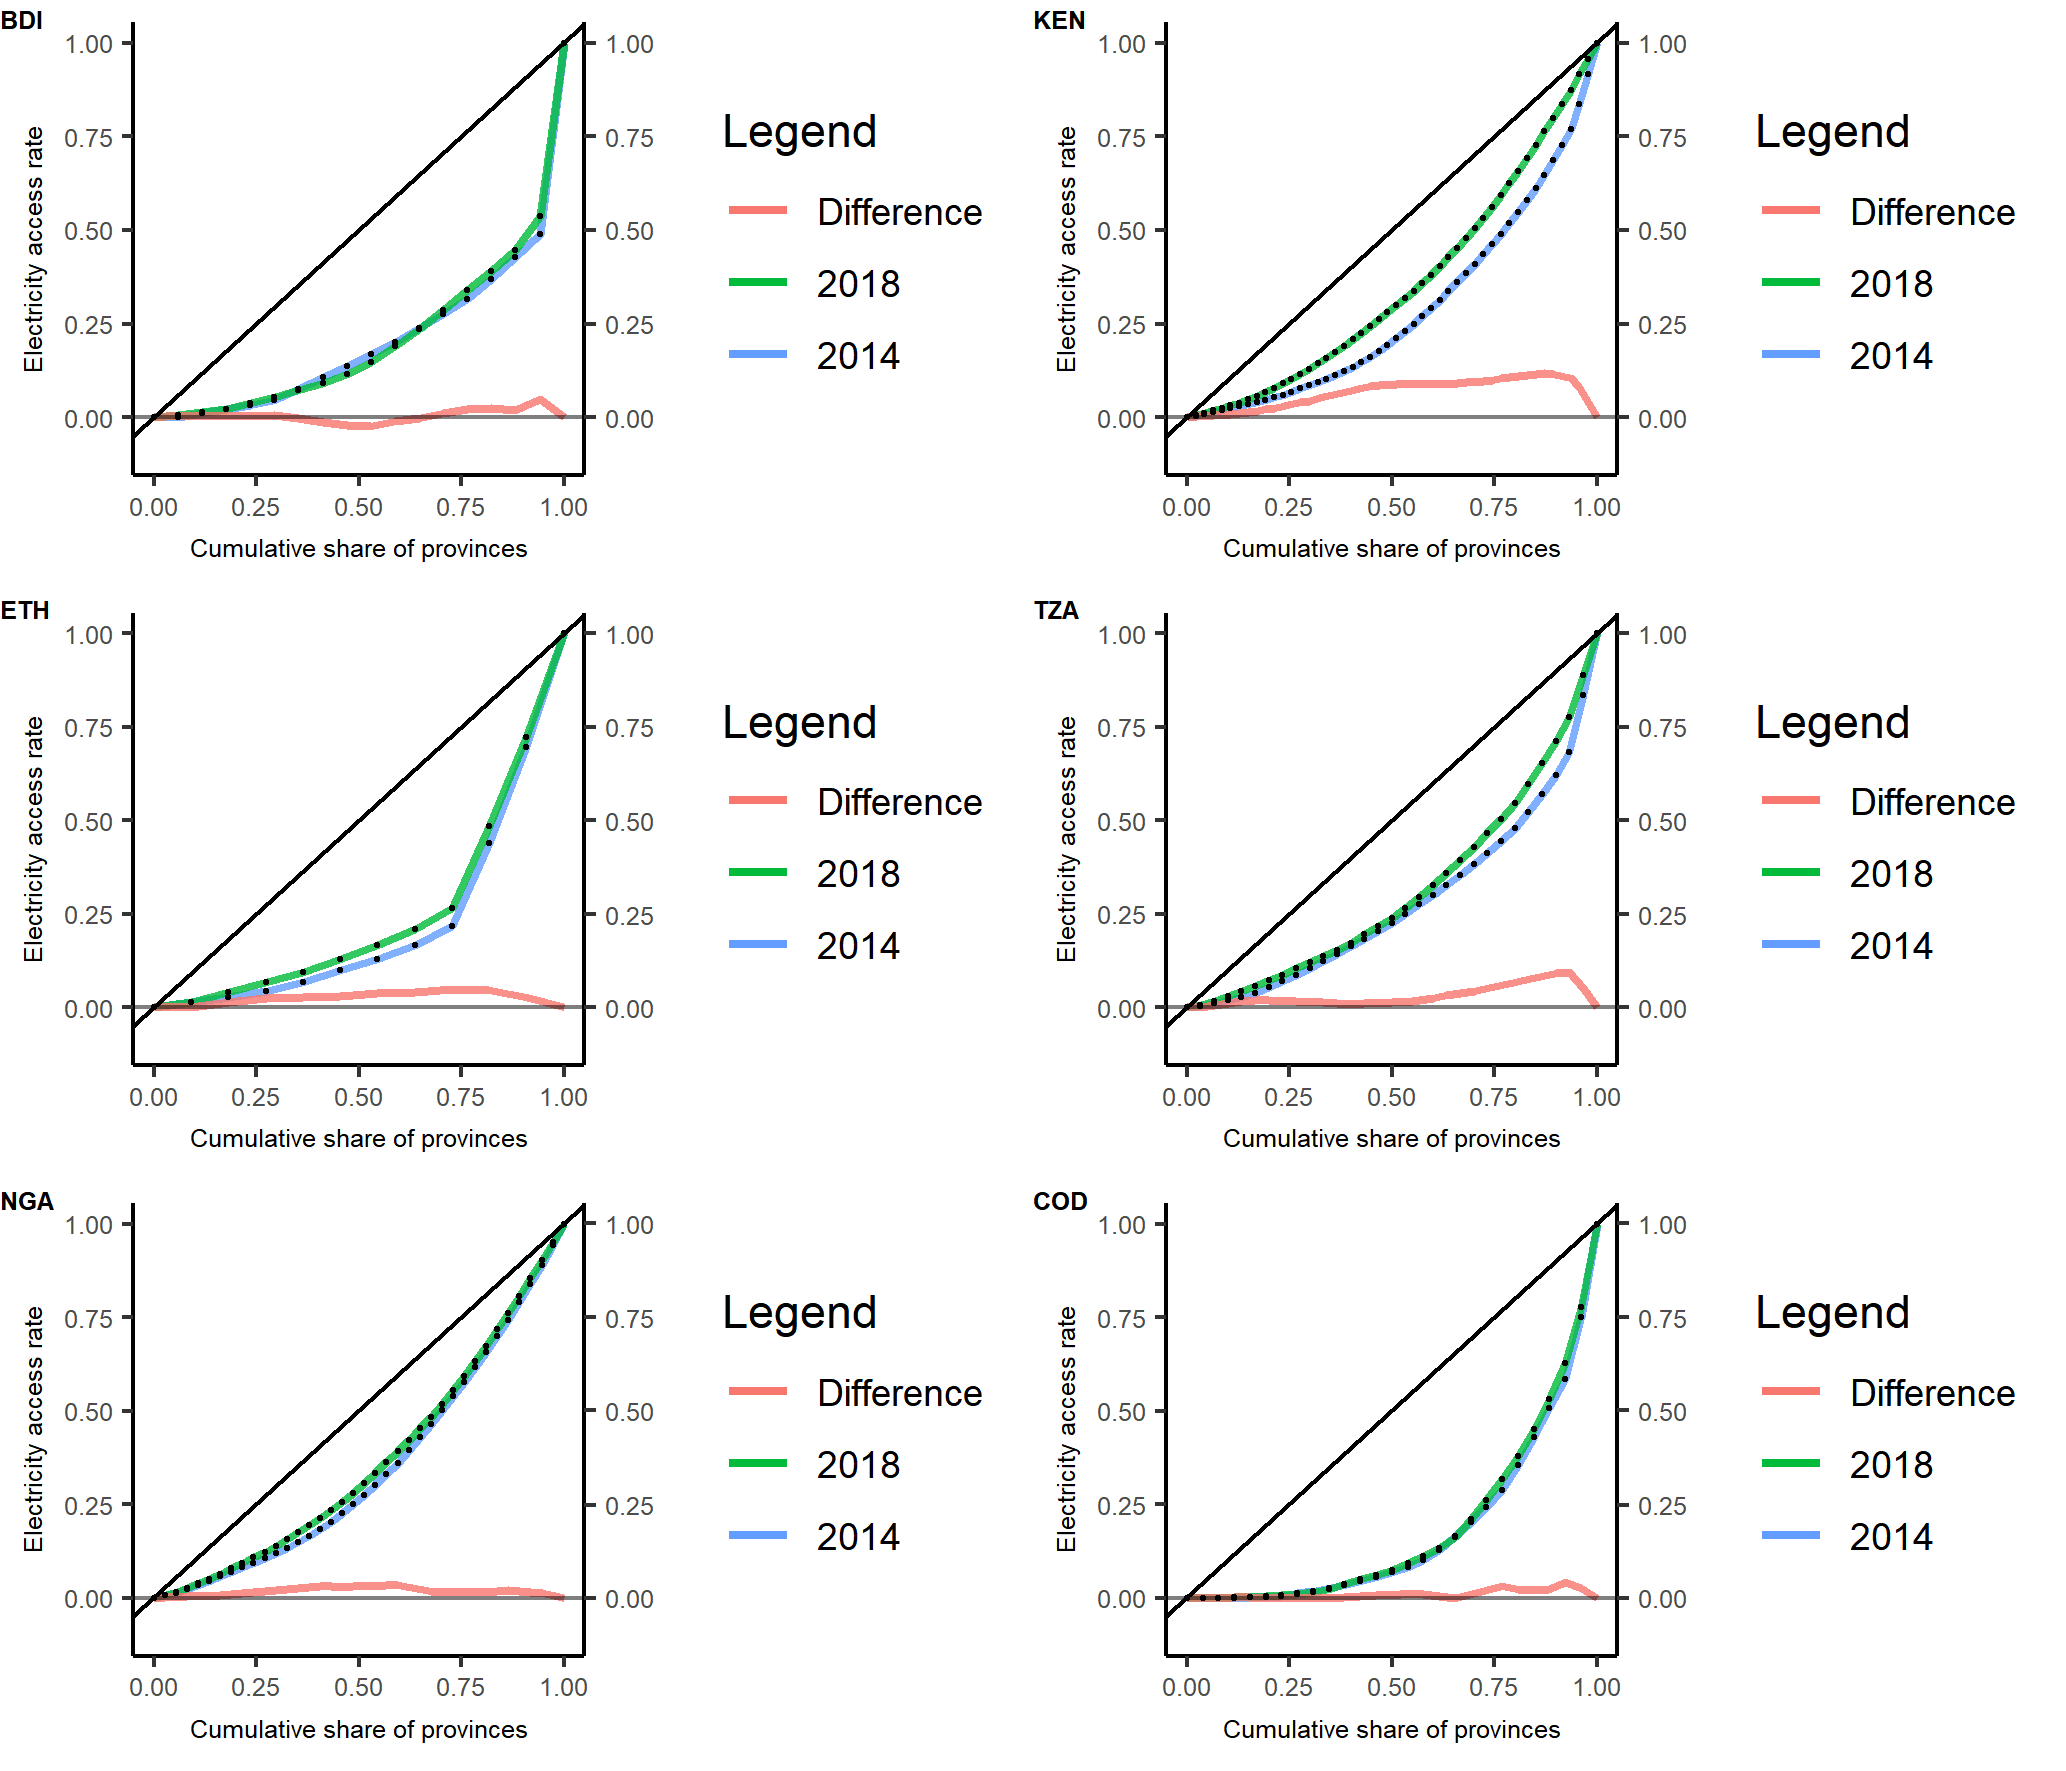
\includegraphics[scale=1]{figures/Lorenz.png} 
    \caption{Lorenz curves compared for selected countries}
    \label{lorenz}
\end{figure}

\subsection{Inequality in residential consumption}
Settlements detected as lit are not necessarily implying a situation of 100\% local electrification, nor that all households are benefiting from the same level of access \citep{riva_merry-go-round_2018}. Here we use the four per-capita light categories (defined as described in Methods) as proxy of electricity residential consumption. We then sum for each province the population that is estimated to have access above/below each tier, a measure that goes beyond the binary access/no-access metric.

Figure \ref{residential_consumption_inequality} shows the within-country split of people living in areas within each per-capita residential consumption category, as defined in the Methods section in rural and urban areas\footnote{Rural and urban areas identification strategy is described in the Methods section}, respectively.

\begin{figure}[H]
    \label{residential_consumption_inequality}
    \centering
    \subfloat[Rural and peri-urban areas ]{{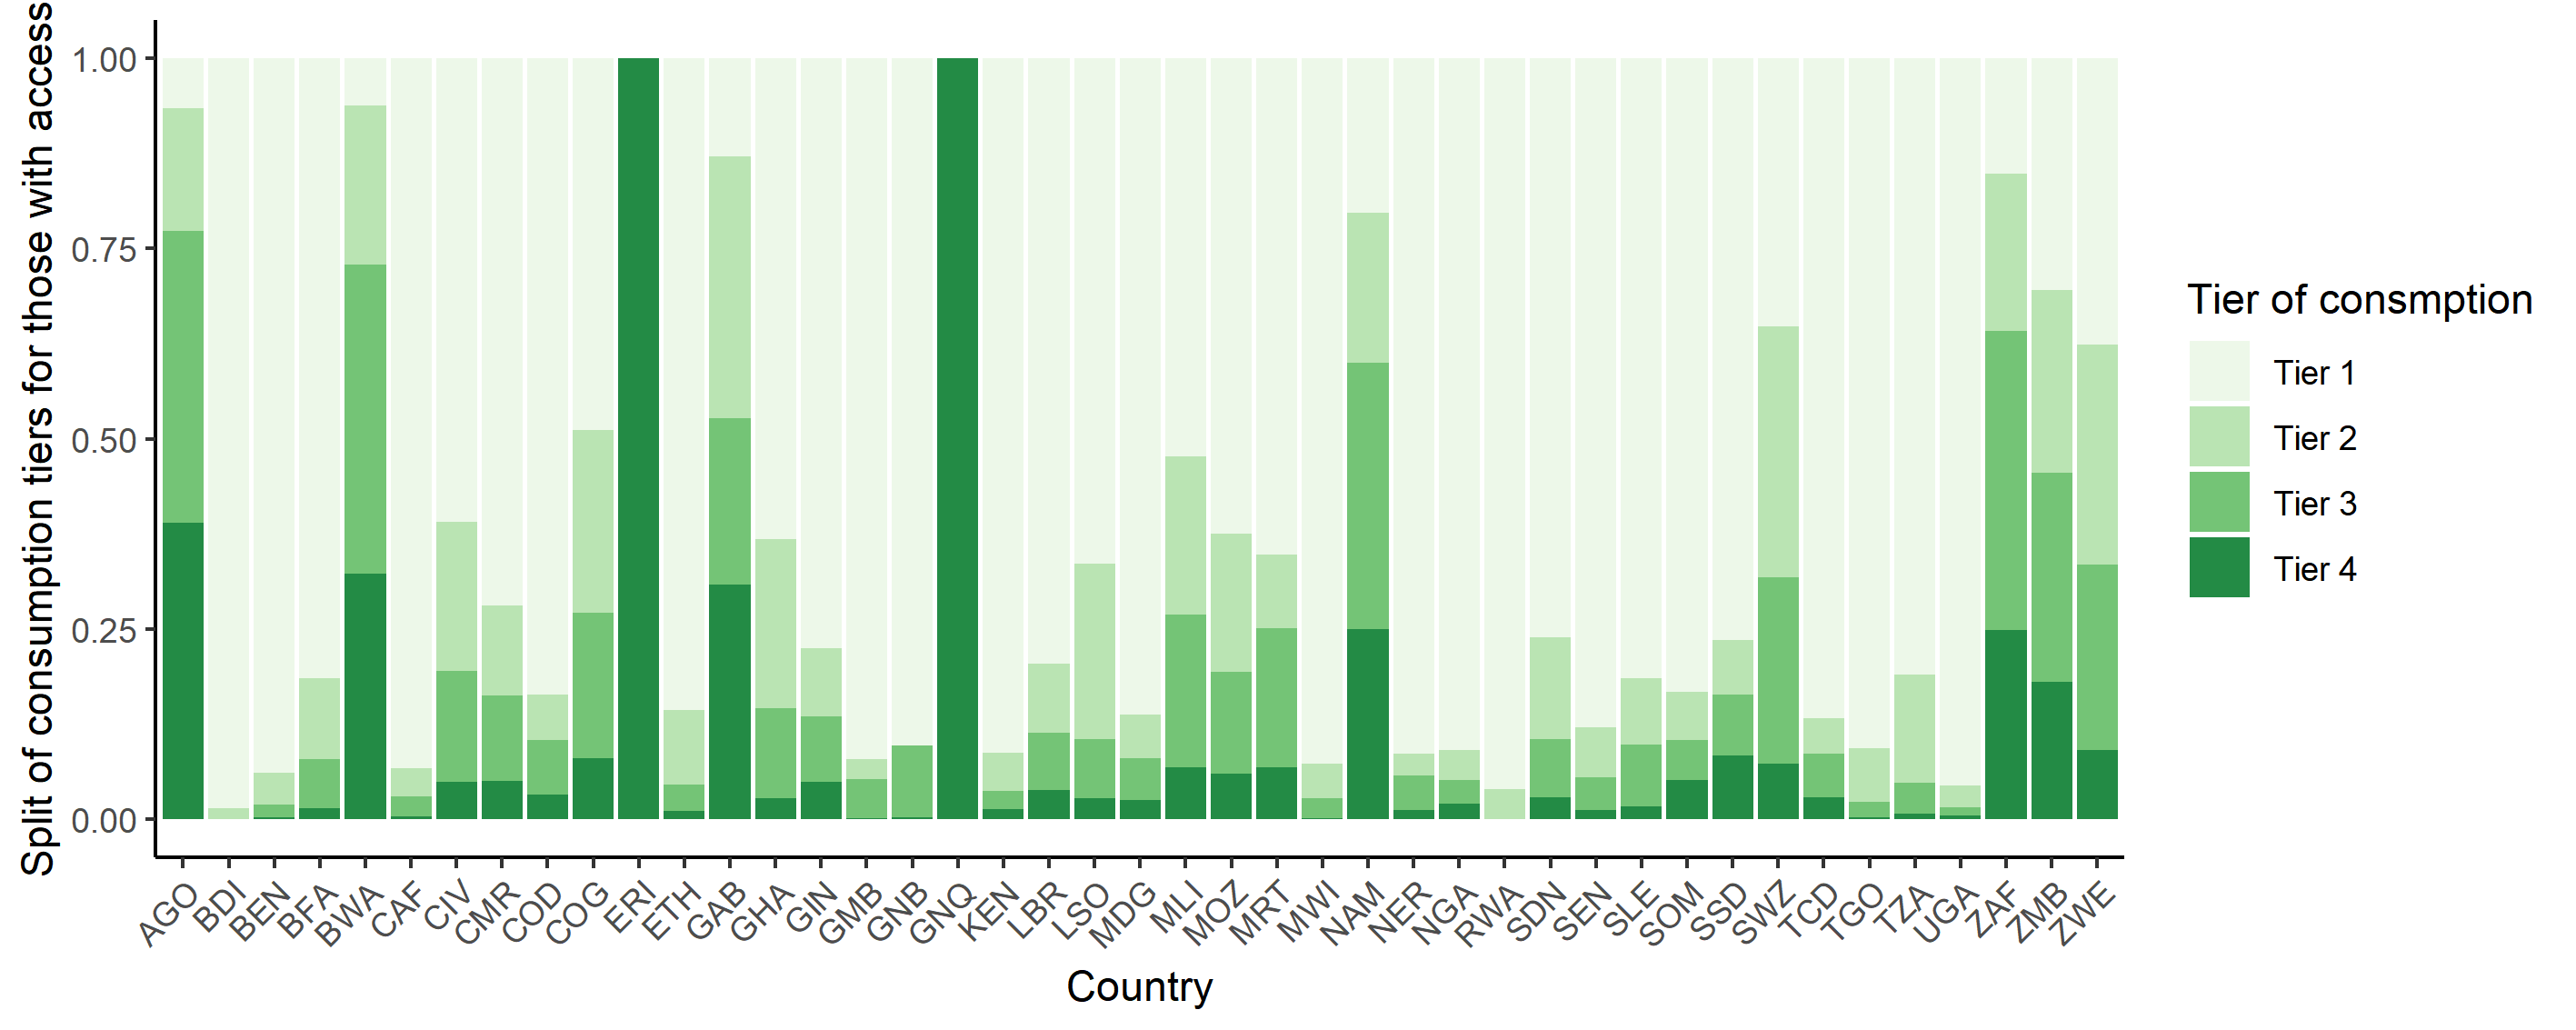
\includegraphics[scale=0.6]{figures/barplot_consumption_rur.png} }}%
    \qquad
    \subfloat[Urban areas]{{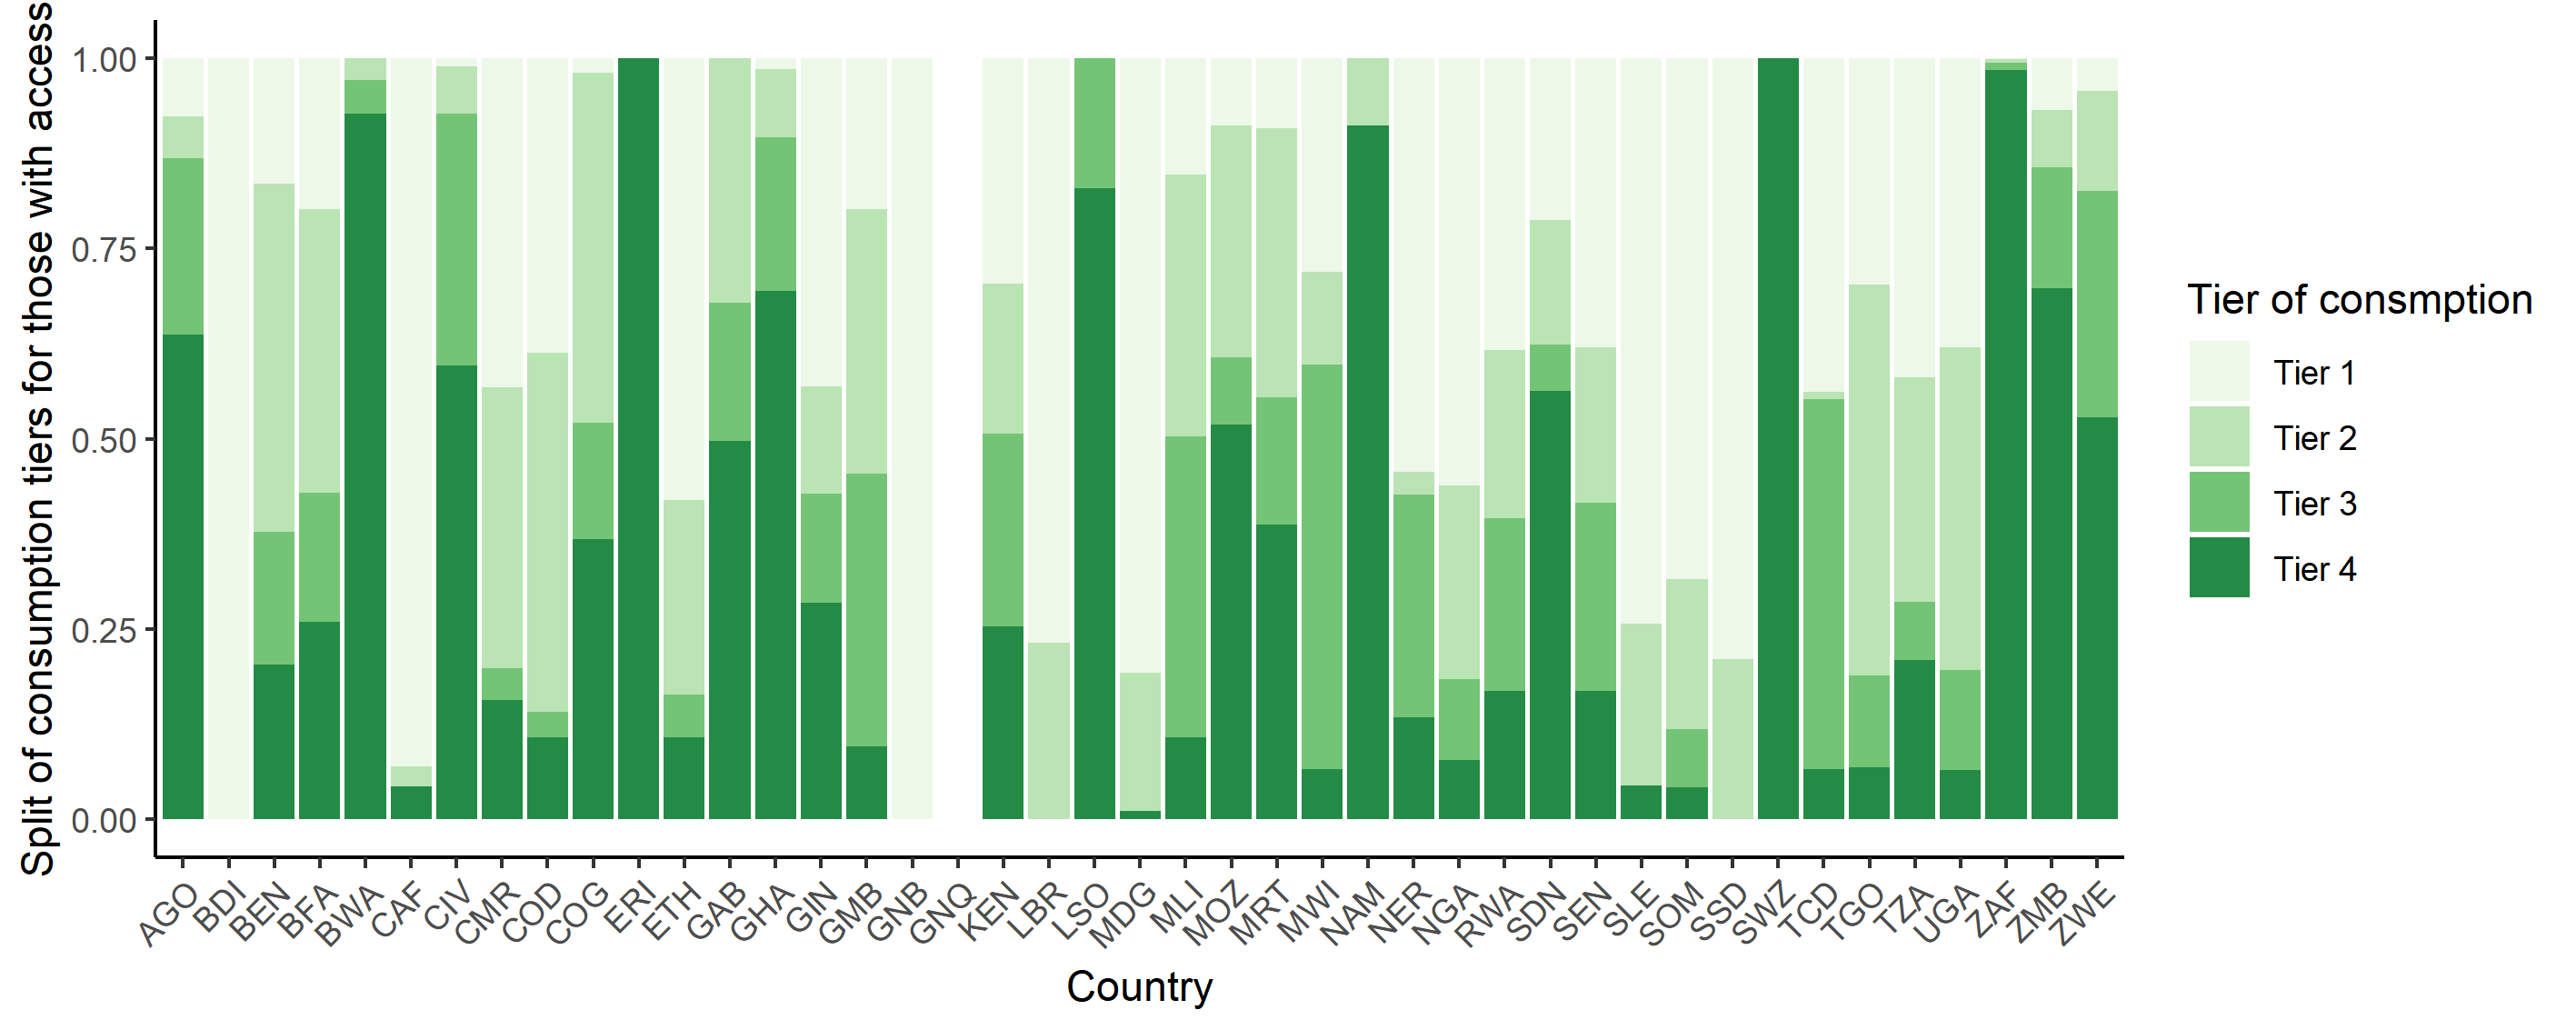
\includegraphics[scale=0.6]{figures/barplot_consumption_urb.png} }}%
    \caption{Barplot of residential electricity consumption tiers split}
\end{figure}

Results show that in rural areas less inequality is found both across and within countries, with Tier 1 representing the bulk of the population in a large number of countries. Exceptions include generally richer countries such as Angola, Botswana, the Republic of Congo, Gabon, Equatorial Guinea, Namibia and South Africa, but also Zambia  or smaller countries like Lesotho and Swaziland. On the other hand, in urban areas only a limited number of countries shows a strong consumption inequality, with little people benefiting from high consumption levels and a very limited minority with higher tiers of consumption. These include Benin, the Central African Republic, the Democratic Republic of the Congo, Ethiopia, Nigeria, Togo, Tanzania, and Uganda. Countries which instead exhibit almost universal Tier-4 urban consumption include - albeit to different degrees - Botswana, Equatorial Guinea, Lesotho, Mozambique, Namibia, Rwanda, Sudan, South Africa, Zimbabwe, and Zambia. 

\subsection{Hotspots identification}
To conclude, here we identify three relevant types of provinces which are relevant to the end of our analysis: (i) the provinces which exhibited a fast growing number of people without access. and thus have contributed the most to limiting the growth in electrification rates over the last five years (Figure \ref{map1}); (ii) provinces where it is plausible to assume that significant latent demand\footnote{Latent demand is defined as that part of the total demand for electricity which cannot be satisfied because of supply, income, or infrastructure constraints.} exists, defined as predominantly rural provinces with high levels of electricity access but low estimated per-capita consumption (Figure \ref{map2}); (iii) rural and urban provinces that experienced the fastest change in the sum of light intensity, here identified as residential electricity demand growth hotspots (Figures \ref{distribution}a-b). 

\begin{figure}[H]
    \centering
    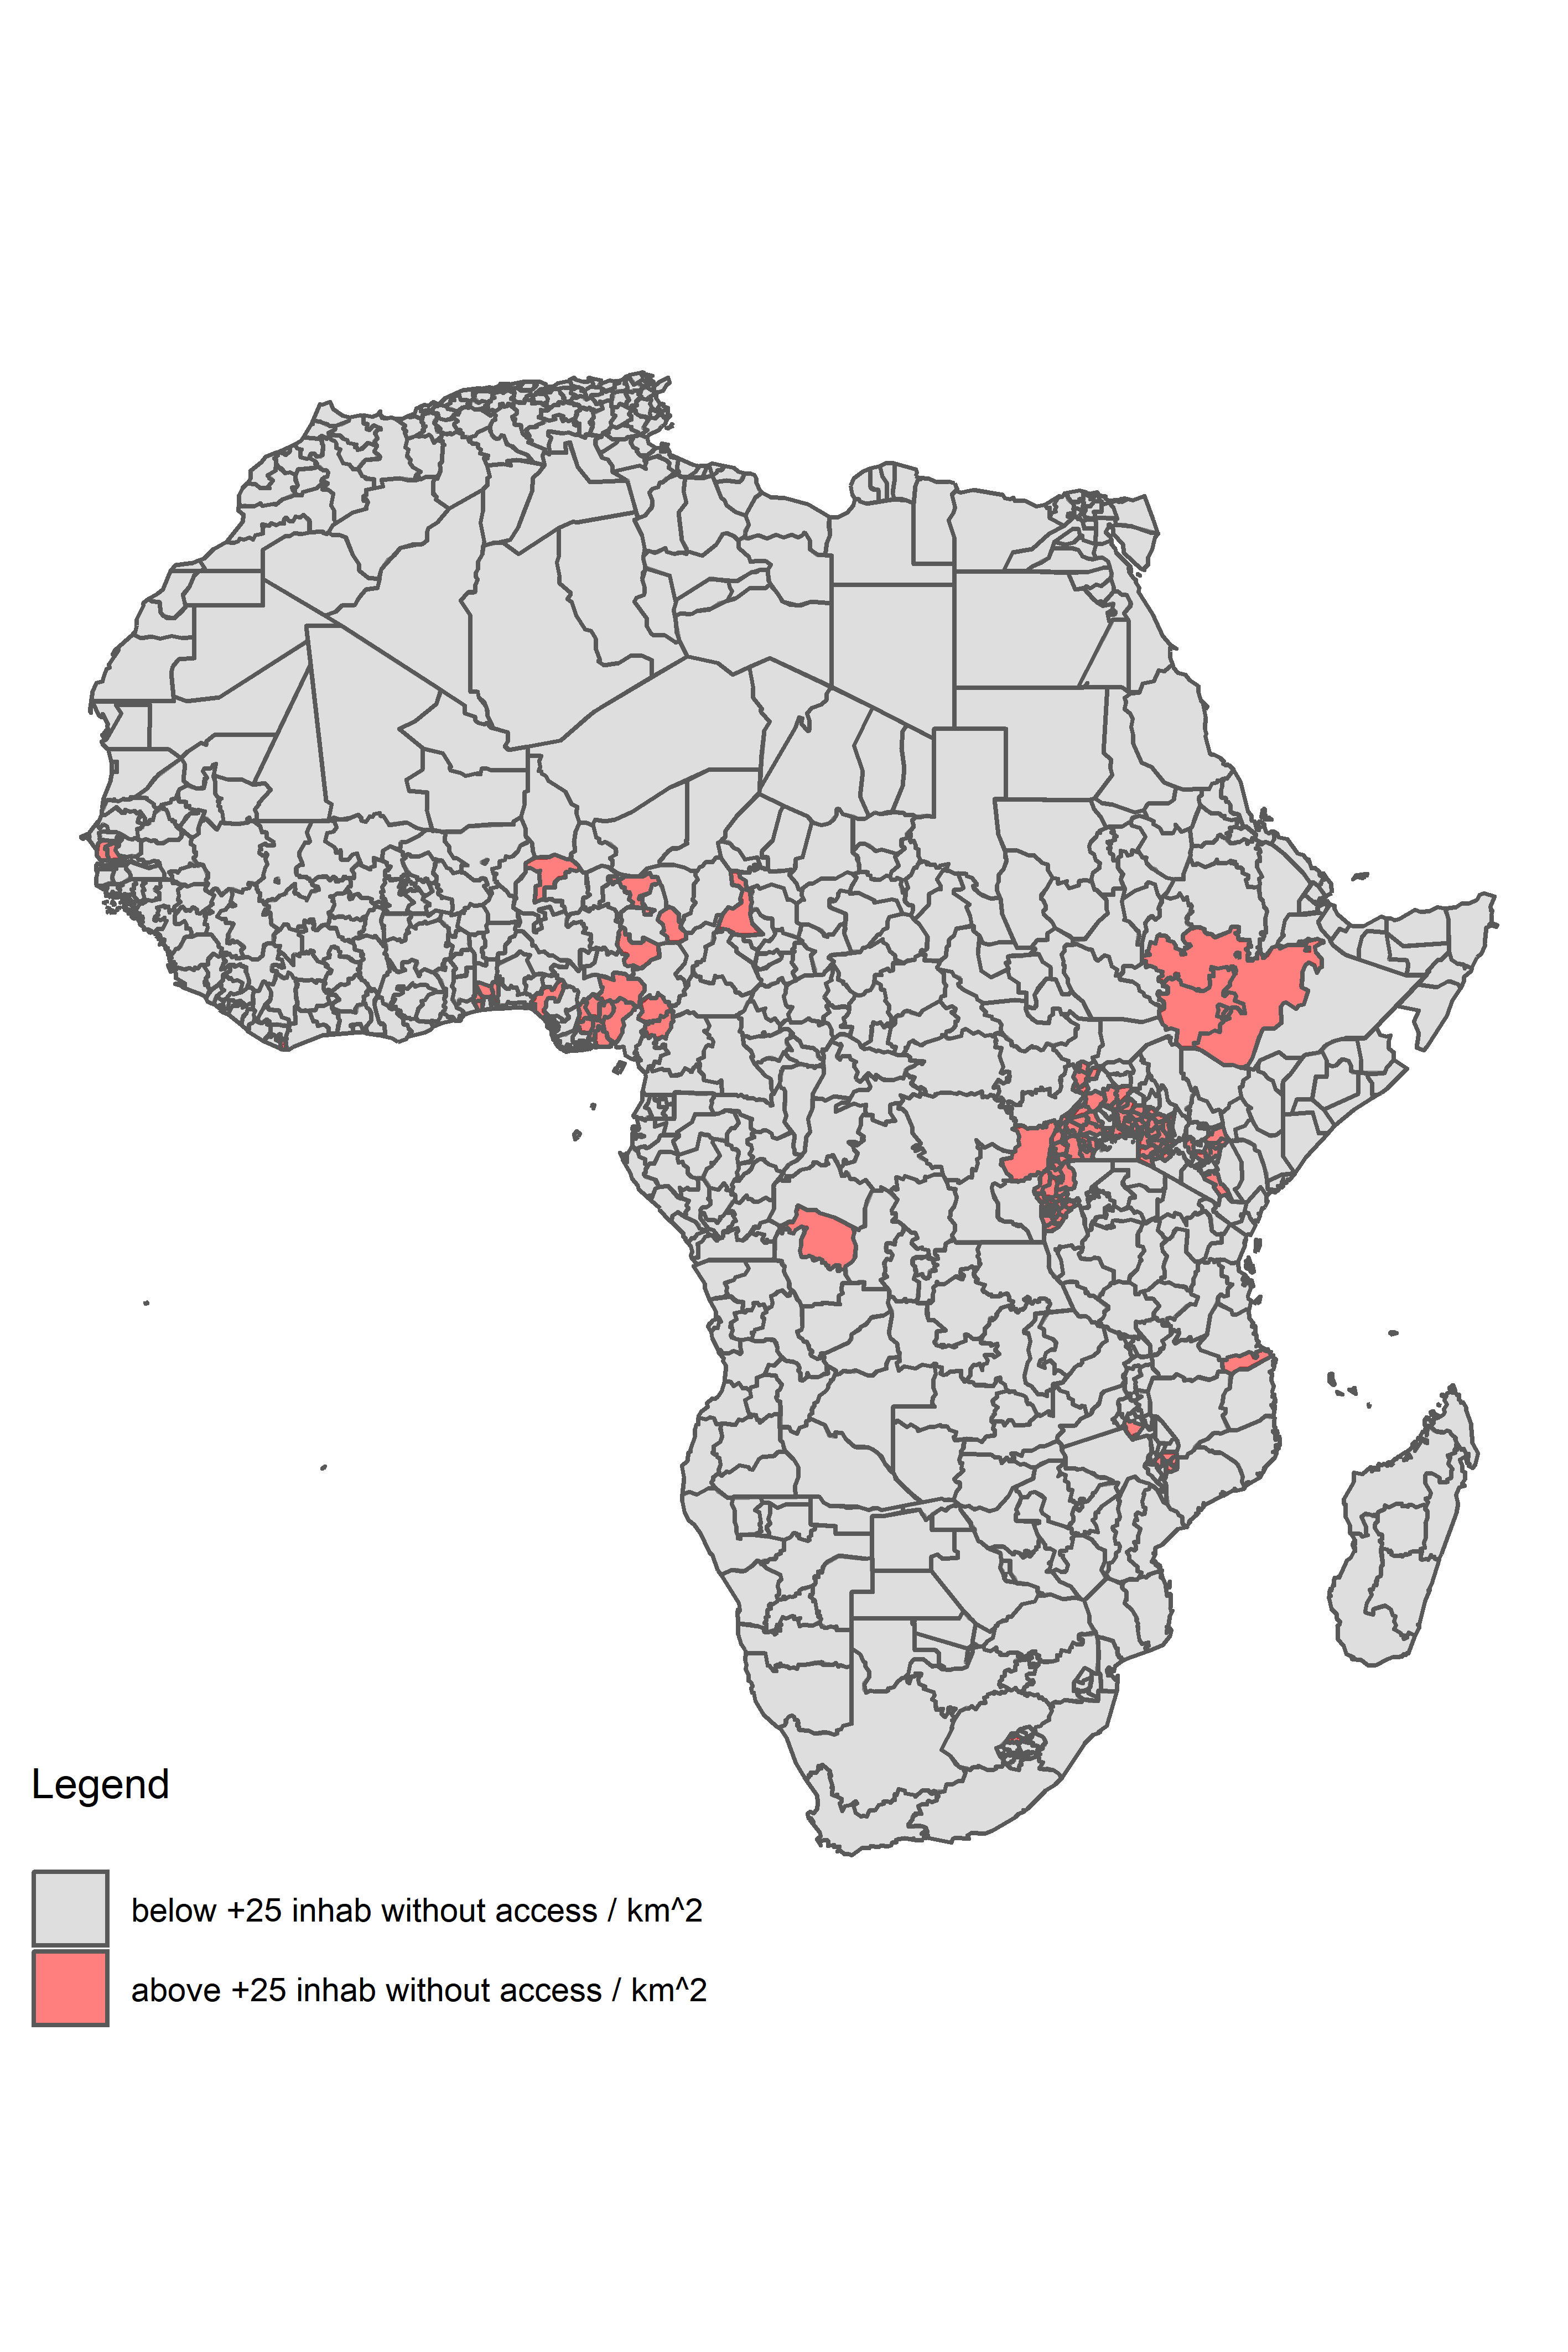
\includegraphics{figures/map1.png}
    \caption{Hotspots with fastest growing number of people without access}
    \label{map1}
\end{figure}

\begin{figure}[H]
    \centering
    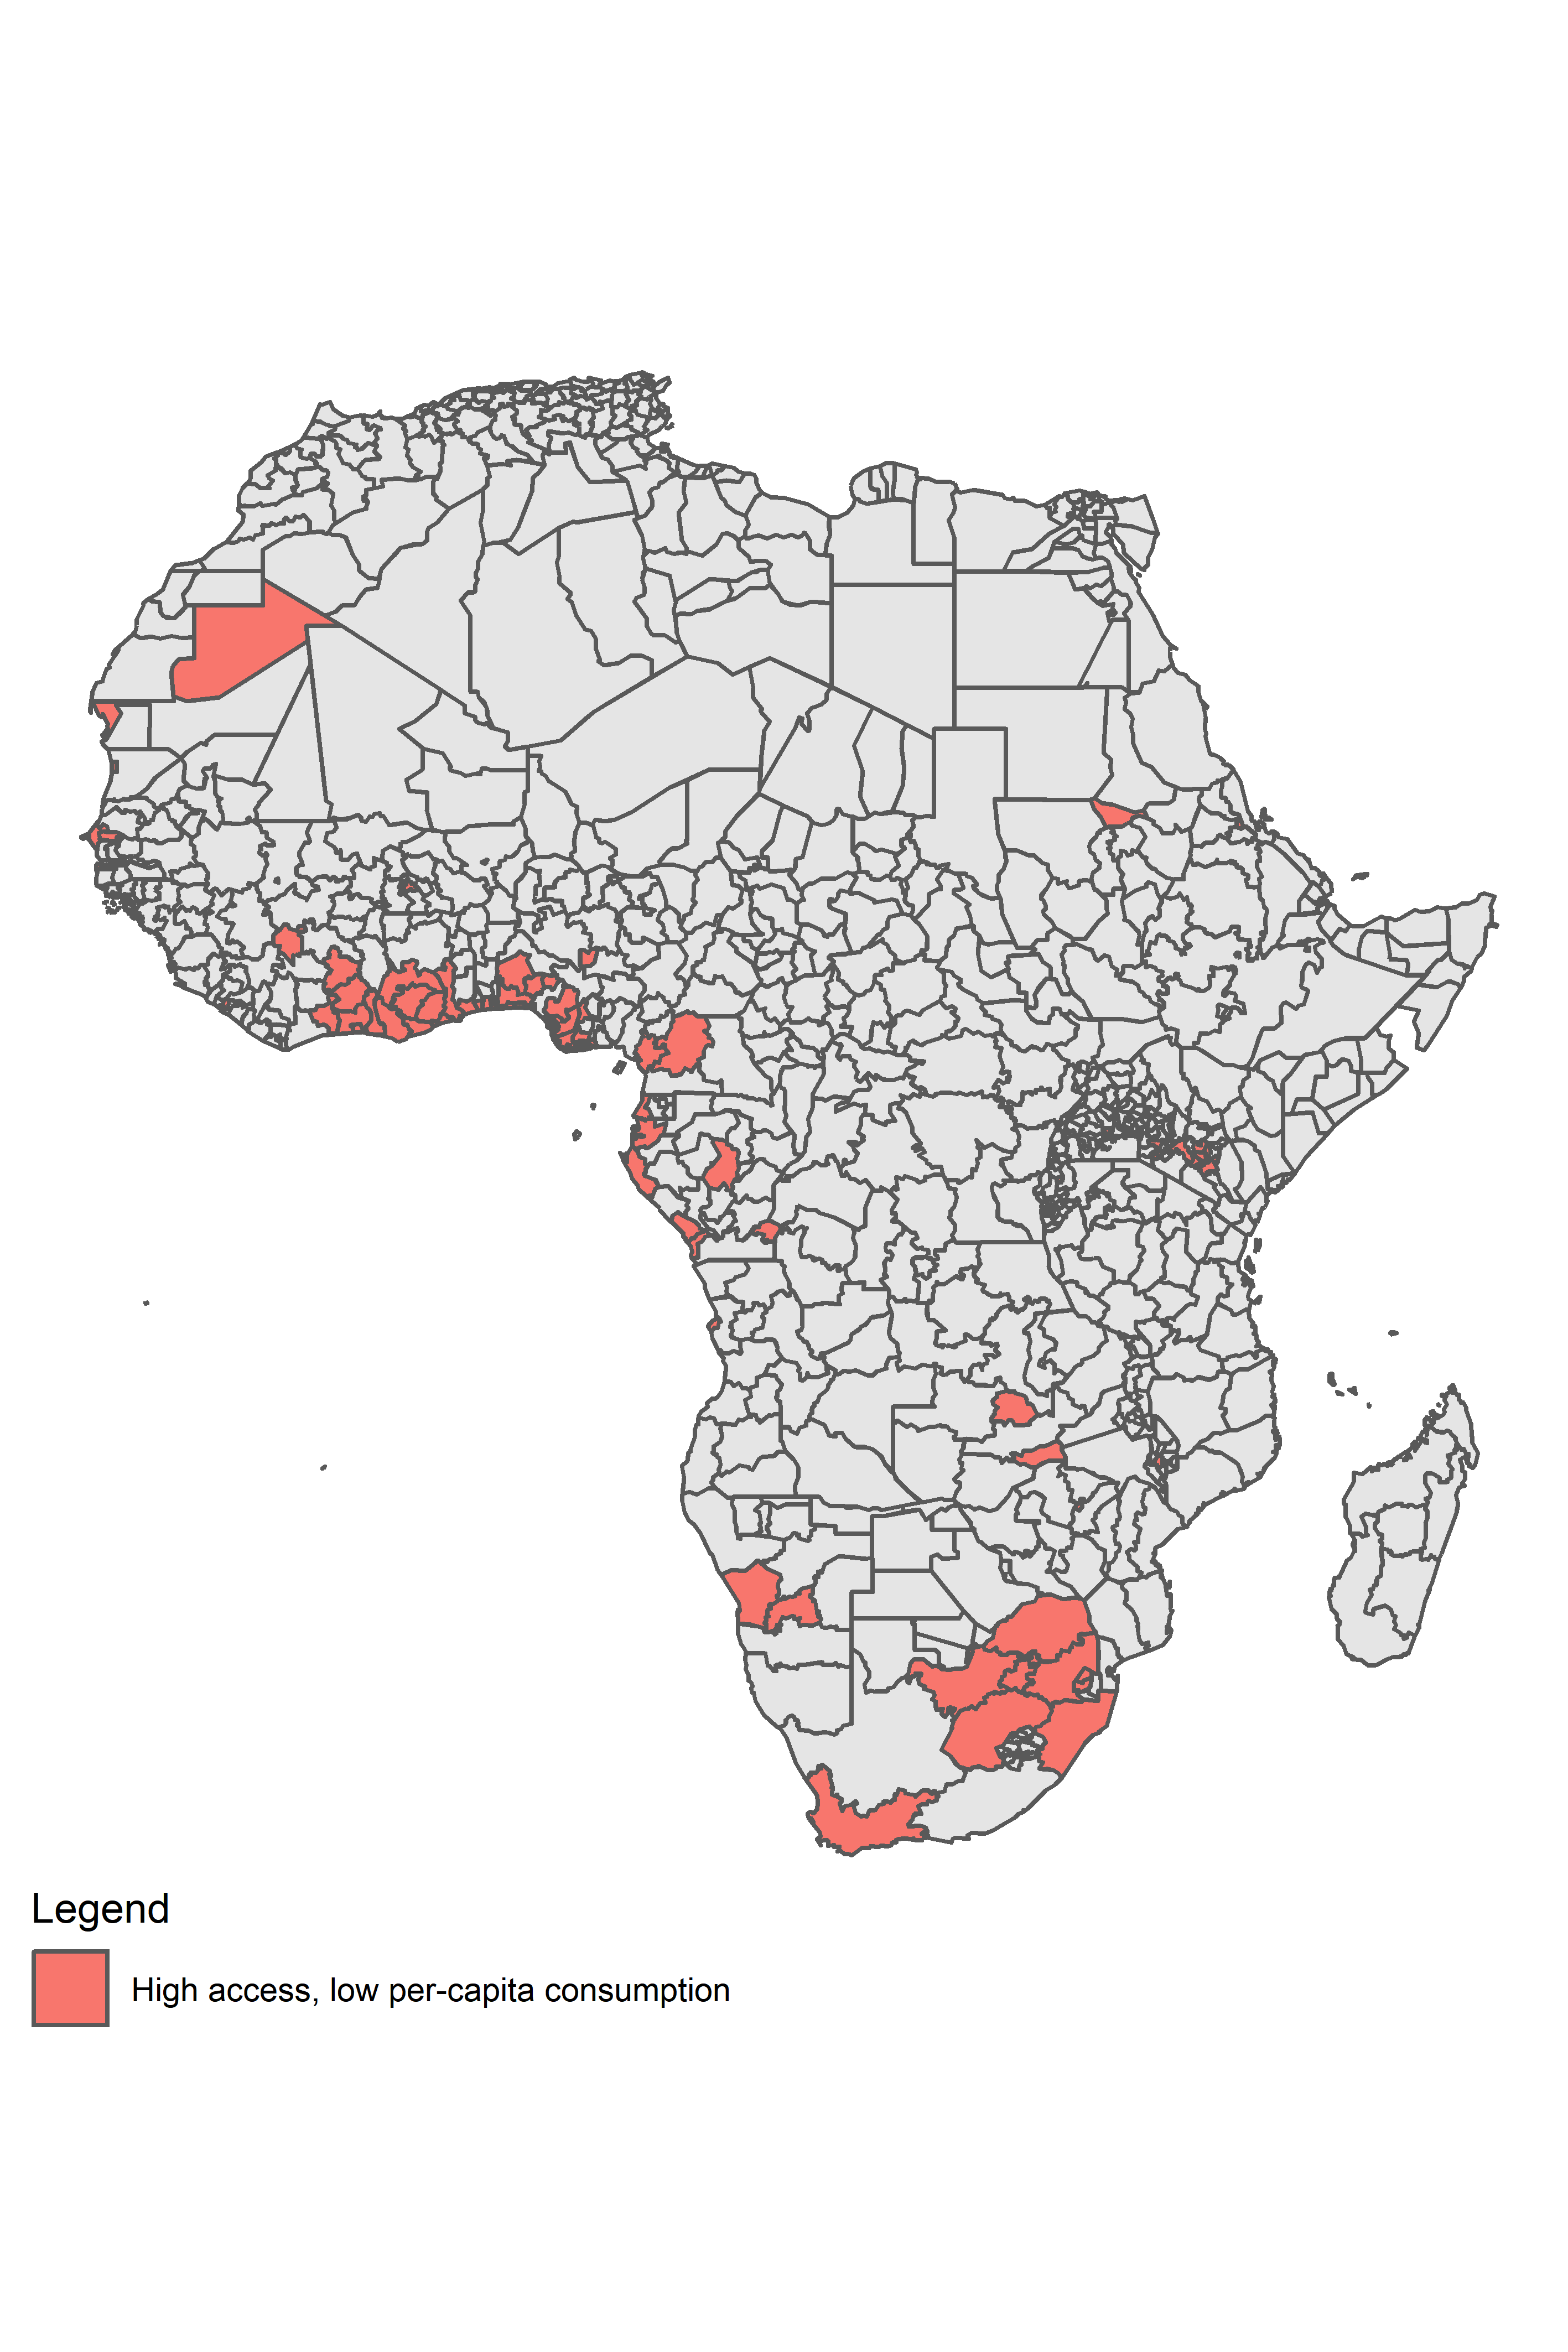
\includegraphics{figures/highaccesslowconsumption.png}
    \caption{Hotspots with fastest growing number of people without access}
    \label{map2}
\end{figure}

\begin{figure}[H]
    \centering
    \subfloat[Urban]{   {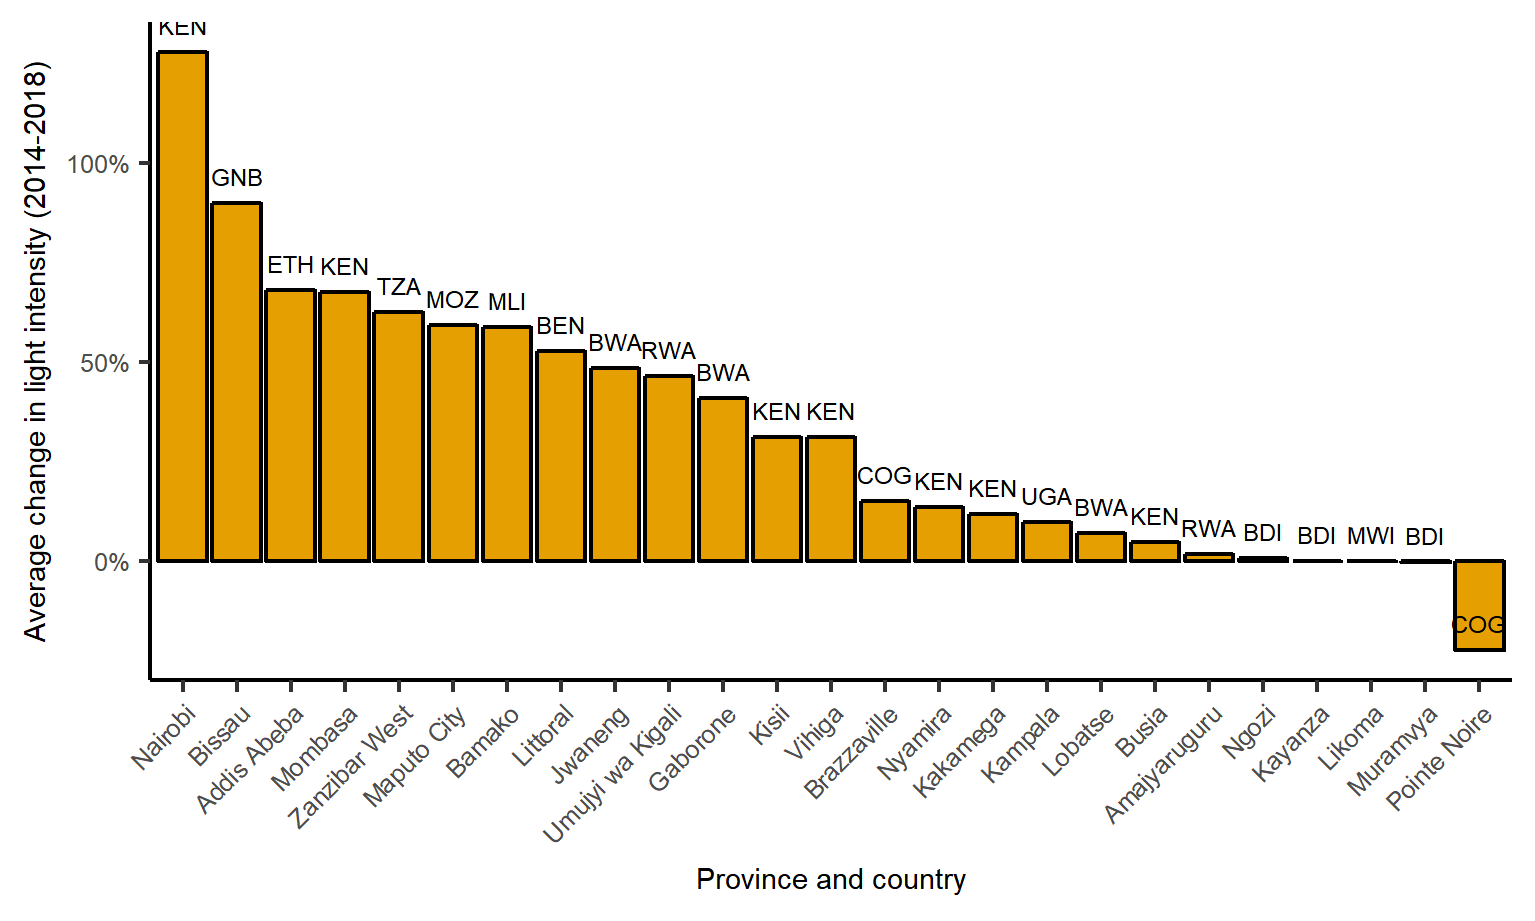
\includegraphics[scale = 1]{figures/change_urban.png} }}%
    \qquad
    \subfloat[Peri-urban and rural]{   {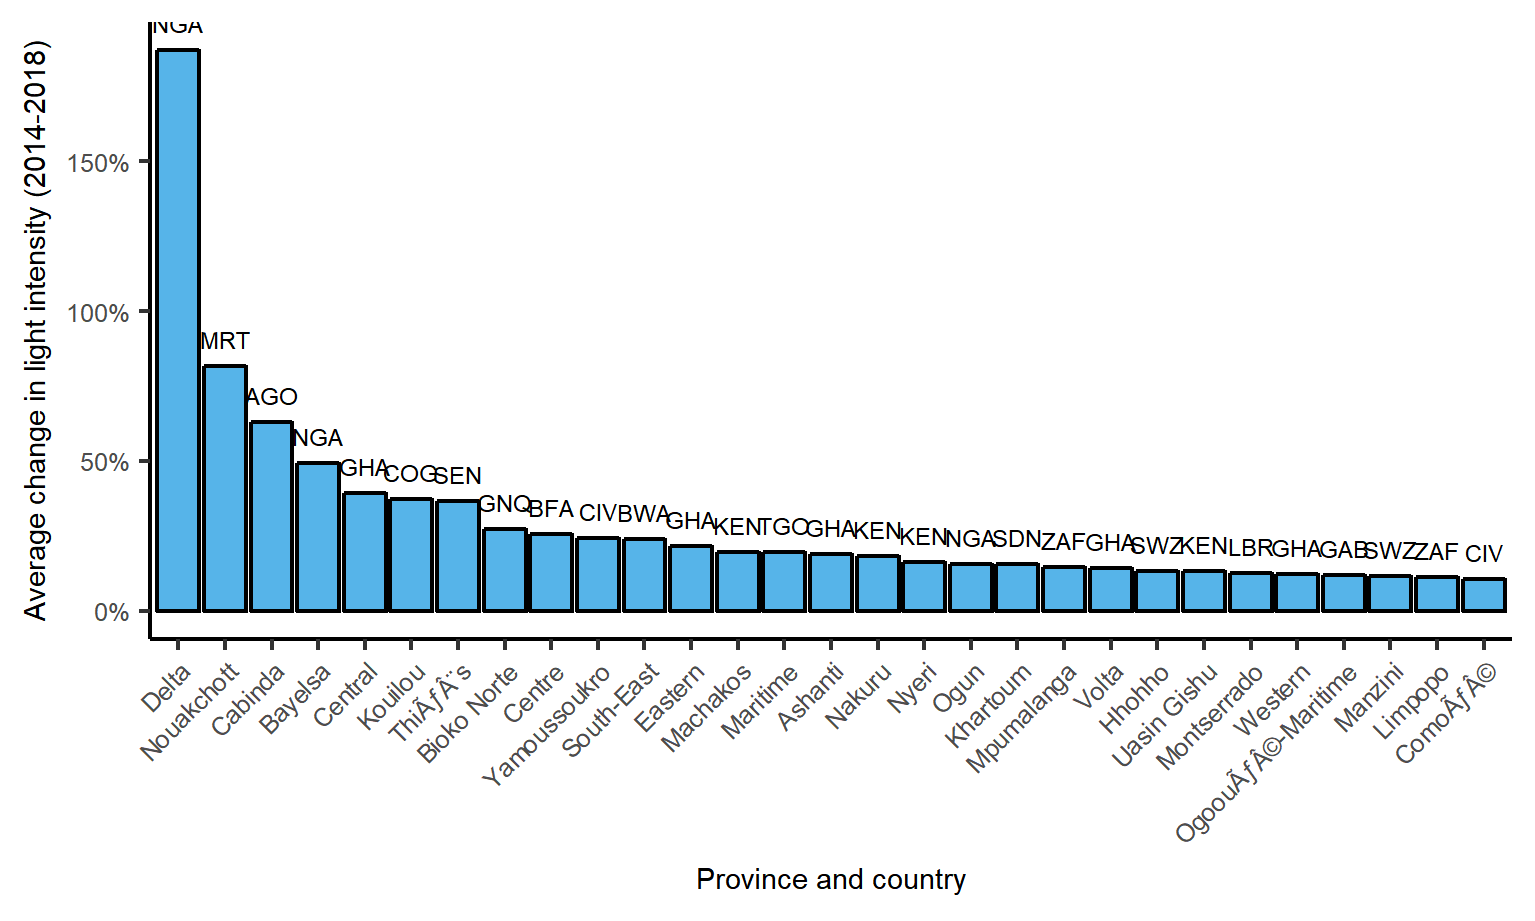
\includegraphics[scale = 1]{figures/change_rural.png} }}%
    \caption{Urban and rural provinces with fastest change in sum of light intensity}
    \label{distribution}
\end{figure}

\section{Discussion}
We introduced a new, updatable, fully-reproducible $1 km^2$ resolution electrification dataset for Sub-Saharan Africa based on gridded datasets, and we showed that it is generally capable of predicting national and province level electrification data from household surveys and national statistics. 

The analysis based on the data has shown that electrification is a complex concept, and that national electrification rates fail to capture an array of dimensions relevant to the achievement of SDG 7, including consumption levels and latent demand in the consumption level of households \citep{poblete-cazenave_income_nodate}. These factors could perpetrate income inequality (the relevant literature has assessed issues of reliability and their negative impacts on small and medium businesses \citep{cole2018power, gannon2018business}) and - potentially - urban migration even under a scenario where universal access in terms of having a generation option available has been attained. 

Policies oriented at achieving SDG 7 of electricity access should therefore attempt at promoting investments which are capable of providing a decent level of electricity consumption, and plan infrastructure so as to make it scalable to subsequent demand growth with income \citep{bazilian_energy_2012}

Grid-connection charges - along with other barriers \citep{lee_barriers_2014} - can play a significant adverse effect in this sense, even for households under cover of the existing national grid, and should therefore be mitigated with smart payment schemes \citep{golumbeanu_connection_2013} and business models. 

Decentralised energy solutions are forecasted to be the least-cost option to bring electricity to households currently without access in a large number of locations across SSA \citep{dagnachew_role_2017}. Nonetheless, their limited supply capability could drive latent demand and increase inequality. System dynamics has proven an insightful approach to the issue \citep{riva_merry-go-round_2018}. 

Overall, we encourage electrification projects and monitoring initiatives to consider a broad array of aspects and implications of electrification, and not to exclusively focus on maximising electrification rates. In this sense, we have shown that high-resolution gridded data can be an effective, low-cost approach to keep track of electrification. 

\section*{Data Access}
The latest version of the data, the code and guide for reproduction, and the interface source code are hosted at \url{https://github.com/giacfalk/Electrification_SSA_data}.

\section*{Supplementary figures}
\renewcommand{\thefigure}{A.\arabic{figure}}
\setcounter{figure}{0}


\section*{Competing interests}
The authors' declare no conflicts of interest. 

\section*{Authors' contributions}

\section*{Acknowledgement}
Support from the MIUR (Italian Ministry of University and Research) through the Catholic University of Milan and to Fondazione Eni Enrico Mattei is gratefully acknowledged. The authors would like to thank Olha Danylo and Edward Byers (IIASA) for their precious inputs.

\section*{References}
\begin{footnotesize}
\bibliography{biblio}
\end{footnotesize}
\end{document}
